\chapter{Background}
\label{chapter:background}

This chapter reviews some general concepts needed to understand the rest of the paper. First, the concept of stability is explained, and several methods used to prove stability are presented. This section is followed by a brief description of the dynamical model of the manipulator. Lastly, several indirect force control methods are introduced, such as impedance and admittance control.

\section{Stability}

The concept of stability is often explained using the example of a ball in a hilly landscape. A stable system can be represented by a ball placed in a valley. When this ball is disturbed (i.e., carried up the hill), it will always return to the lowest point, also called the equilibrium point, when released. When we now put this ball on top of a hill and disturb it (i.e., give it a push), we will see an unstable system instead. The ball will roll off the hill and never return without us carrying it up again. This stability can be local, only valid in a region around the equilibrium point or global and valid for all system states. In control theory, stability means that the control is guaranteed to always converges to a given setpoint while staying bounded in state space. This setpoint can be any arbitrary quantity like position, angle, velocity, effort, rotational speed, or voltage. In the case of a regularisation task, this setpoint can be static, but it can also move in time for trajectory tracking or manipulation tasks.

Multiple general methods have been designed to investigate the behaviour and stability of linear systems. Since a general closed-loop solution exists for a linear system, a simple eigenvalue analysis of this solution can be used to determine stability. The stability type and boundaries can be further investigated using frequency domain mathematical techniques like the Laplace transform, Fourier transform, z-transform, Bode plots, root locus, and Nyquist stability criterion \cite{bacciottiStabilityControlLinear2019}. Because a linear system only has one equilibrium point, it is always globally stable or unstable. On the other hand, no general closed-loop solution is available for nonlinear systems and determining stability is not trivial. Furthermore, nonlinear systems can also have multiple equilibrium points, meaning that stability can only be investigated locally around an equilibrium point and only under some conditions is global.

Lyapunov's stability theory, first introduced in 1892, provides a way to reason about the stability of equilibrium points of linear and nonlinear systems without solving the complete system behaviour. It consists of several notions of stability, fundamental theorems and methods that can be used to investigate the system's stability. Lyapunov's stability theory can be applied to both autonomous and non-autonomous systems. Below, several notions of stability for autonomous systems will be discussed, followed by methods that can be used to prove the stability of equilibrium points. After that, these notions and methods will be extended to unforced non-autonomous time-dependent systems. In doing so, the concept of boundedness, which is used for systems with no clear equilibrium point, and methods for dealing with perturbed systems are presented. Lastly, input-state stability and passivity will be introduced to investigate the stability of forced non-autonomous systems.

\subsection{Stability of autonomous systems}

\subsubsection{Stability notions}
% NOTE: The equations in this section come from \cite{khalilNonlinearSystems2002, mullenLectureNonlinearSystems}.

The introduction of Lyapunov's stability theory resulted in several new stability notions. The most used in the impedance literature are stability (and its absence, instability), asymptotic stability, and exponential stability.

%% FIGURE - Stability notions.
\begin{figure}
  \centering
  \begin{subfigure}{0.31\textwidth}
    \centering
    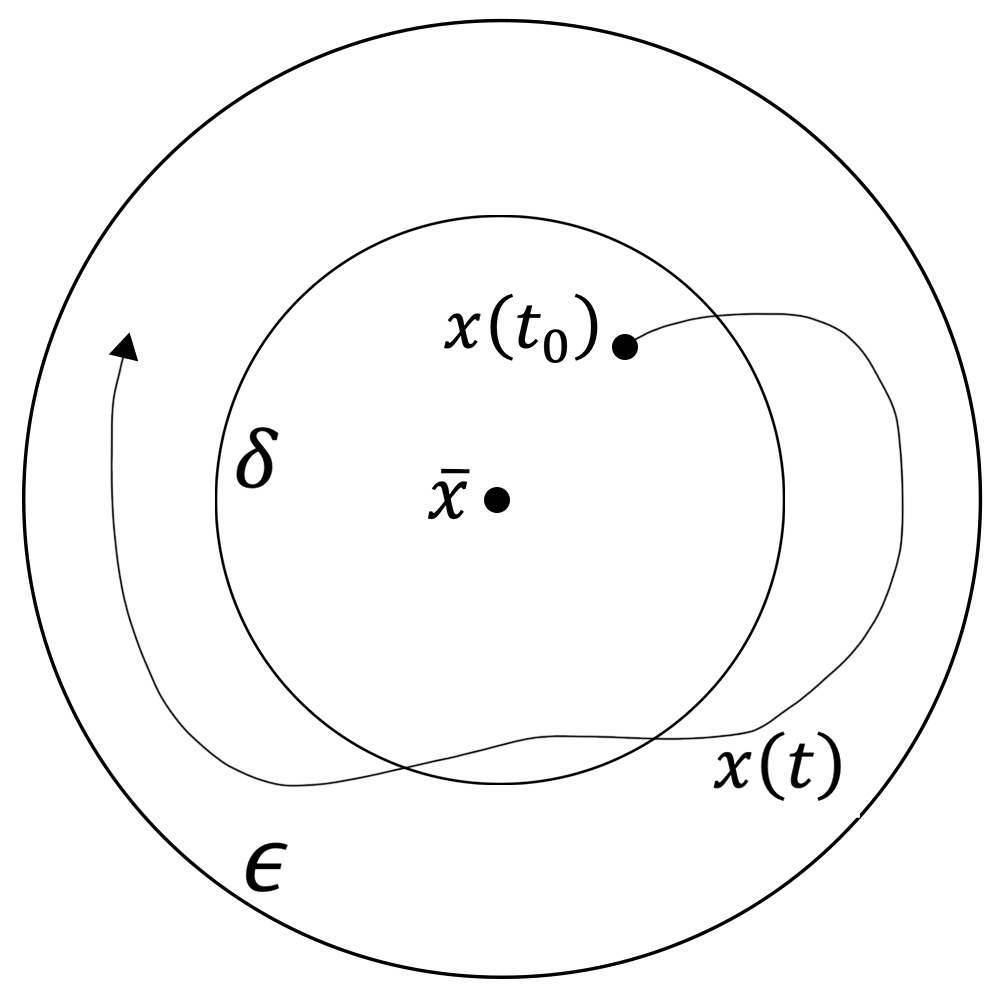
\includegraphics[width=\linewidth]{figures/figure-SISL.jpg}
    \caption{Stability in the sense of Lyapunov} \label{fig:SISL}
  \end{subfigure}
  \hspace*{\fill} % Maximize separation between the subfigures.
  \begin{subfigure}{0.31\textwidth}
    \centering
    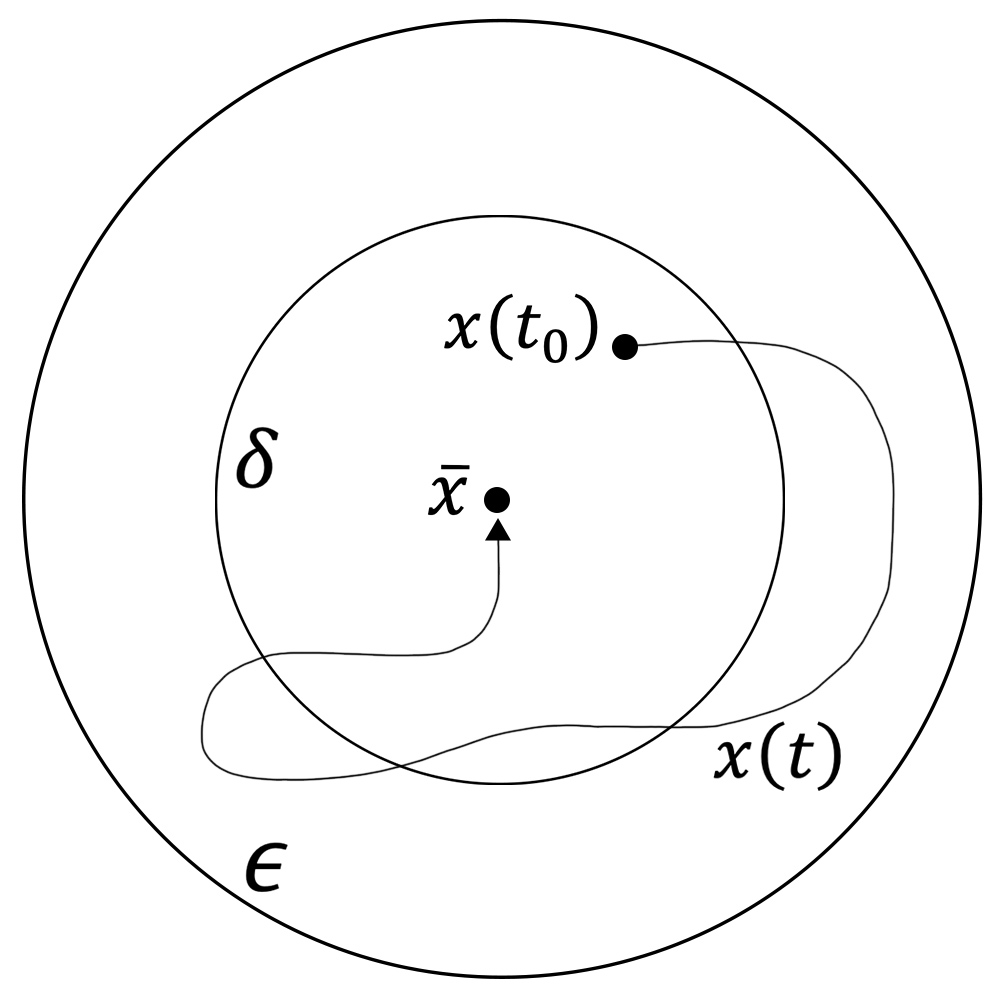
\includegraphics[width=\linewidth]{figures/figure-AS.jpg}
    \caption{Asymptotic stability} \label{fig:AS}
  \end{subfigure}
  \hspace*{\fill} % Maximize separation between the subfigures.
  \begin{subfigure}{0.31\textwidth}
    \centering
    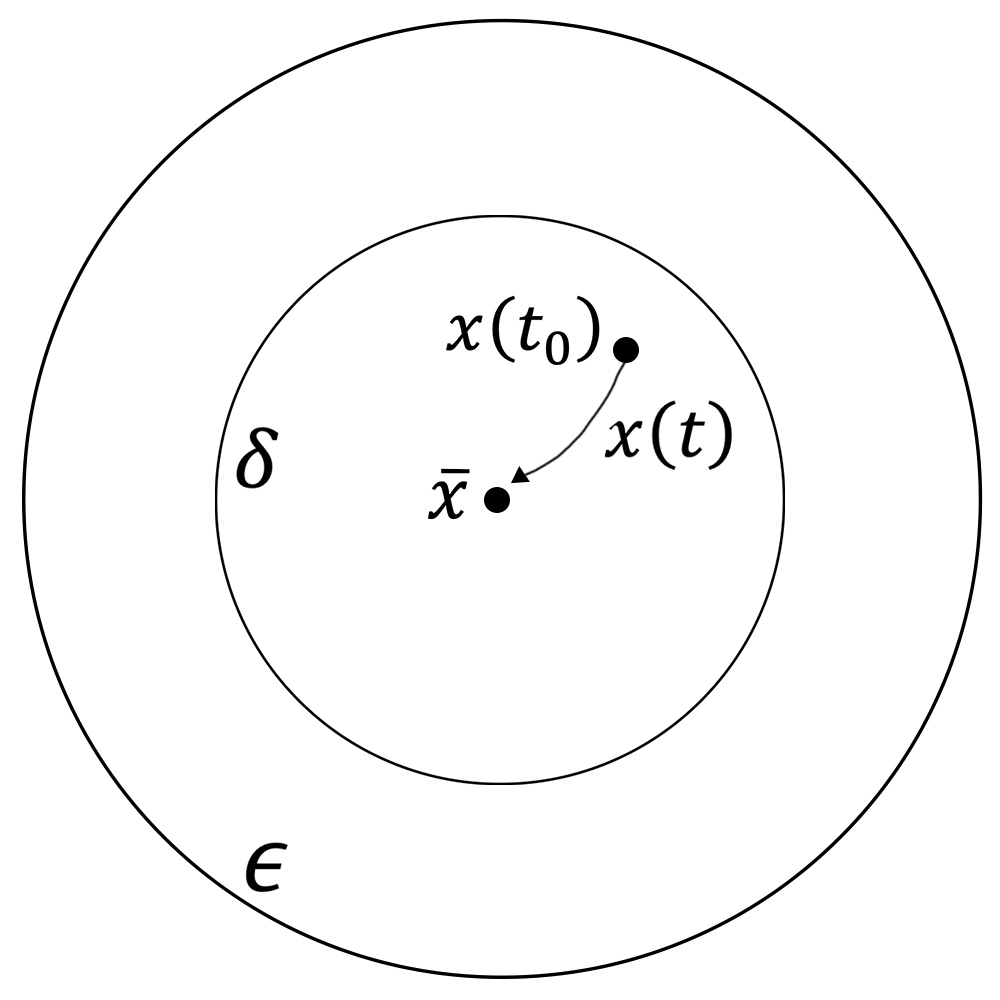
\includegraphics[width=\linewidth]{figures/figure-ES.jpg}
    \caption{Exponential stability} \label{fig:ES}
  \end{subfigure}

  \caption[Several notions of stability.]{Several notions of stability. In these figures, $\delta$, $\epsilon$ represent the start and end stability bounds, $\bar{x}$ the equilibrium point, and $x\left(t_0\right)$ and $x\left(t\right)$ the initial point and trajectory, respectively.} \label{fig:stability_notions}
\end{figure}

\paragraph{Stability in the sense of Lyapunov}

In Lyapunov's stability theory, stability is concerned with the trajectories' behaviour rather than the equilibrium point's stability. This notion of stability is handy since a noise or disturbance can always perturb a physical system from its equilibrium. Although, as shown in the following chapters, Lyapunov's theory can also be extended to work with specific non-autonomous systems, let us, for simplicity, consider the following autonomous nonlinear system:
\begin{equation} \label{eq:auto_nonlinear_system}
  \dot{x} = f\left(x\right),
\end{equation}
where $f : D \rightarrow\mathbb{R}^n$ is a locally Lipschitz map from a domain $D \subset \mathbb{R}^n$ into $\mathbb{R}^n$. An equilibrium point of this system $\bar{x}$ is \textbf{stable in the sense of Lyapunov (SISL)} if, for each $\epsilon > 0$, there exists some $\delta > 0$ such that:
\begin{equation}
  \left\| x\left(t\right) - \bar{x} \right\| < \epsilon, \quad \forall \; t \ge t_0,
\end{equation}
whenever $\left\| x\left(t_0\right) - \bar{x} \right\| < \delta$. Intuitively this means that any trajectory starting inside circle $\delta$ will never leave circle $\epsilon$ (see figure \ref{fig:SISL}). Since SISL is not a global condition, $\delta$ and $\epsilon$ should be chosen as small as possible to provide the most robust bounds. Logically, every system that does not adhere to these conditions is \textbf{unstable}.

\paragraph{Asymptotic stability}

A stricter notion of stability called asymptotic stability can be created by imposing some additional conditions. An equilibrium point $\bar{x}$ is \textbf{asymptotically stable (AS)} if:
\begin{itemize}
  \item It is SISL.
  \item Some $\delta > 0$ exists such that when $\left\| x\left(t_0\right) - \bar{x} \right\| < \delta, \quad \lim_{t \to \infty} \left\| x\left(t\right) - \bar{x} \right\| = 0$.
\end{itemize}
Intuitively this means that the trajectory will always converge to $\bar{x}$ if started inside circle $\delta$ (see figure \ref{fig:AS}). If $\delta = \infty$, the system is called \textbf{globally asymptotically stable (GAS)}.

\paragraph{Exponential stability}

Lastly, an equilibrium point $\bar{x}$ is \textbf{exponentially stable (ES)} with rate of convergence $\alpha$ if:
\begin{itemize}
  \item It is SISL.
  \item There exists a $M, \lambda > 0$ such that $\left\| x\left(t \right) \right\| \leq Me^{-\lambda\left(t-t_0 \right)}\cdot \left\| x\left(t_0\right) \right\|$.
\end{itemize}
The intuition for this type of stability is like asymptotic stability, but now the trajectory exponentially converges to the equilibrium point (see figure \ref{fig:ES}). Since this results in a stricter condition, exponential stability implies asymptotic stability, but the converse does not always hold. If $\delta = \infty$, the system is called \textbf{globally exponentially stable (GES)}.

\subsubsection{Stability methods}

Based on these new stability notions, two general stability methods were designed to investigate the stability of (non-)linear systems: \textbf{Lyapunov's indirect} and \textbf{Lyapunov's direct method}.

\paragraph{Lyapunov's indirect method}

Lyapunov's indirect method linearises the system using a first-order Taylor series around an equilibrium point. After this linearisation, the techniques developed for linear systems can be used to conclude the stability of the nonlinear system at the equilibrium point \cite{vidyasagarNonlinearSystemsAnalysis2002}. Although this method provides an easy way to investigate the local stability of an equilibrium point of both autonomous and non-autonomous time-dependent systems, it is only valid in a small region around this point. Therefore, it cannot give any conclusions about the global stability of the nonlinear system or the region of attraction of an equilibrium point (i.e., the set of states for which the system converges to the equilibrium point as $t \rightarrow \infty$).

\paragraph{Lyapnov's direct method}

Lyapunov's direct method takes a different approach by investigating the stability of a system using an energy-based method. Doing this provides sufficient conditions for the local stability of an equilibrium point without investigating the full system dynamics. In some cases, it also allows for conclusions about the global system stability and can estimate the region of attraction \cite{khalilNonlinearSystems2002}. Let us first introduce the intuition behind this method using the example of a simple damped pendulum (see example \ref{ex:pendulum}).

%% EXAMPLE - Pendulum.
% NOTE: Example below is adapted from example 9.1 of https://underactuated.mit.edu/lyapunov.html.
\begin{example}{Simple damped pendulum energy investigation.}{pendulum}
  \begin{center}
    \captionsetup{type=figure}
    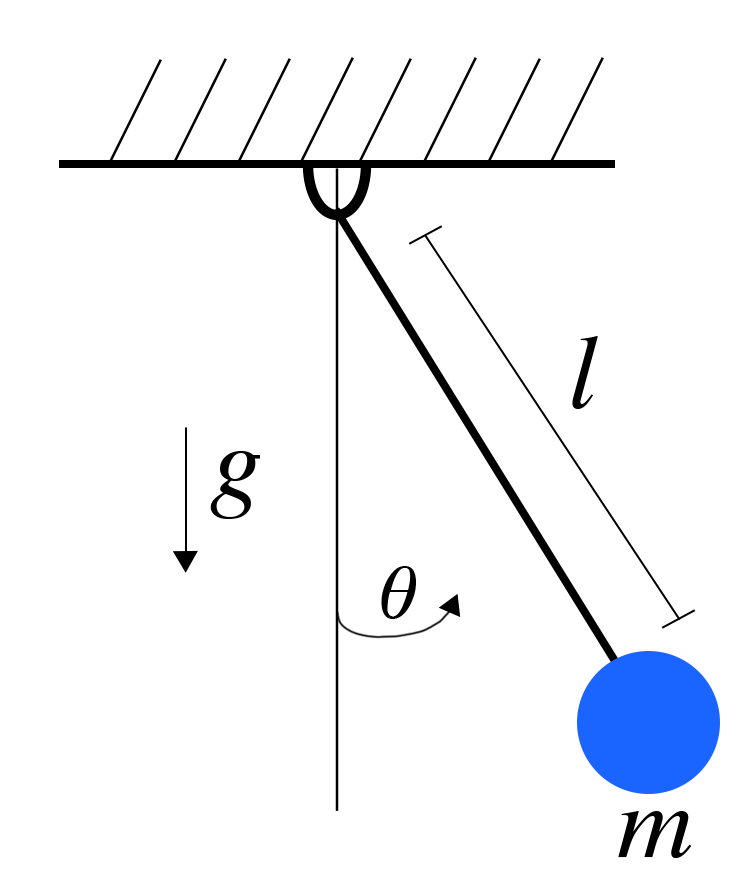
\includegraphics[width=0.3\linewidth]{figures/figure-pendulum.png}
    \captionof{figure}[Simple damped pendulum.]{Simple damped pendulum. In this figure, $m$, $l$, and $\theta$ are the pendulum's mass, length, and angle, and $g$ and $b$ are the gravity constant and damping coefficient, respectively.} \label{fig:pendulum}
  \end{center}

  Let us investigate the stability of the pendulum found in figure \ref{fig:pendulum} above. The equations of motion of this simple damped pendulum are given by
  \begin{equation} \label{eq:pendulum}
    ml^2\ddot{\theta} + mgl\sin{\theta} = -b\dot{\theta},
  \end{equation}
  where $m$, $l$, and $\theta$ are the mass, length, and angle of the pendulum and $g$ and $b$\footnote{Some texts like \cite{khalilNonlinearControl2015} use $kl^2$ instead of $b$, where $k$ is the friction coefficient.} are the gravity constant and damping coefficient, respectively. Although a closed-form solution exists for this relatively simple example, it consists of integrating several elliptical integrals and provides us with relatively little intuition. More importantly, a closed-form solution is not guaranteed to exist for a more complicated system. However, from experience, we know that this damped pendulum (with $b > 0$) when released at an angle $\theta_{t_0}$ will lose energy due to air friction and, after some oscillations, will eventually rest at the lowest point, with minimal energy (i.e., $\theta = 2\pi k$). We can use this intuition to prove the stability of the system by looking at its total energy (kinetic + potential), which can be written down as\footnote{The reference position is chosen so that the potential energy is zero at the lowest point.}
  \begin{equation} \label{eq:pendulum_energy}
    E\left(\theta, \dot{\theta}\right) = \frac{1}{2}ml^2\dot{\theta}^2 + mgl(1 - \cos{\theta}).
  \end{equation}
  Evaluating the time derivative of this energy function gives us
  \begin{equation}
    \frac{d}{dt}E = ml^2\dot{\theta}\ddot{\theta} + \dot{\theta}mgl\sin{\theta},
  \end{equation}
  and substituting in the system dynamics from equation \eqref{eq:pendulum} reveals
  \begin{equation}
    \frac{d}{dt}E = -b\dot{\theta} \le 0.
  \end{equation}
  Since this condition ensures that the system's energy will never increase, it is sufficient for proving stability. Unfortunately, since $\theta = 2\pi k$ is not the only minimum for which $\dot{E} = 0$, it does not prove that the system will converge to this minimum. It is also zero when the pendulum changes direction during the oscillating behaviour. However, as shown later, we can use \hyperref[th:lasalles]{La Salle's Invariance principle} to prove convergence.
\end{example}

The example above showed that a relatively simple energy function (i.e., mechanical energy) could be used to say something about the system stability without computing the complex analytical closed-form solution. Lyapunov's direct method generalizes this idea to systems that might not be stable in mechanical energy. It states that a general (non-)linear system is stable if a \textbf{positive definite} (energy) function of the state variables $V\left(x\right)$\footnote{A small positive constant can be added to the energy function in \ref{eq:pendulum_energy} to make it strictly positive definite.}, called a \textbf{Lyapunov function}, exists that decreases with time, meaning $\dot{V}\left(x\right)$ is \textbf{negative (semi-)definite}. These Lyapunov functions, when found, can be used to demonstrate several notions of stability when certain conditions are met. The Lyapunov conditions for the earlier defined stability notions (i.e., SISL, AS, EX) are shown without proof\footnote{The proofs can be found in chapter 4 of \cite{khalilNonlinearSystems2002} and section 3.3 of \cite{khalilNonlinearControl2015}.} in theorem \ref{th:auto_lyapunov_conditions}. In this theorem, the origin (i.e., $x = 0$) is taken as the equilibrium point. However, since any point can be shifted to the origin using a change of variables, it does not lead to a loss of generality.

%% Theorem - Lyapunov stability conditions for autonomous systems.
\begin{theorem}[list text=Sufficient conditions for stability of autonomous systems,after pre=\footnotetext{Theorem 4.1 and 4.10 of \cite{khalilNonlinearSystems2002} and theorem 3.3 \cite{khalilNonlinearControl2015} were slightly adjusted and combined to improve clarity.}]{Sufficient conditions for stability of autonomous systems \cite{khalilNonlinearSystems2002}\footnotemark}{auto_lyapunov_conditions}
  Let $x = 0$ be an equilibrium point of \eqref{eq:auto_nonlinear_system} and $D \subset\mathbb{R}^n$ be a domain containing $x = 0$. Let $V: D \rightarrow \mathbb{R}$ be a continuously differentiable function such that
  \begin{equation} \label{eq:lyapunov_psd_condition}
    V \left( 0 \right) = 0 \quad \textrm{and} \quad V \left( x \right)> 0 \quad \textrm{in} \quad D -\left\{ 0 \right\}
  \end{equation}
  \begin{equation}
    \dot{ V }\left( x \right) = \frac{\partial V}{\partial x} f \left( x \right)\le 0 \quad \textrm{in} \quad D
  \end{equation}
  then, $x = 0$ is (locally) \textbf{SISL}. Moreover, if
  \begin{equation} \label{eq:lyapunov_AS_condition}
    \dot{ V }\left( x \right) = \frac{\partial V}{\partial x} f \left( x \right)< 0 \quad \textrm{in} \quad D - \left\{ 0 \right\}
  \end{equation}
  then $x = 0$ is (locally) \textbf{AS}. Furthermore, if we have
  \begin{equation} \label{eq:lyapunov_ES_condition}
    \dot{ V }\left( x \right) = \frac{\partial V}{\partial x} f \left( x \right)\le- \alpha V \left( x \right) \quad \textrm{in} \quad D - \left\{ 0 \right\}
  \end{equation}
  then $x = 0$ is (locally) \textbf{ES}. Finally, if $D = R^n$, and \eqref{eq:lyapunov_psd_condition} holds for all $x \neq 0$, and $x$ is
  \begin{equation}
    \left\| x \right\| \rightarrow \infty \Rightarrow V\left(x\right) \rightarrow \infty
  \end{equation}
  then $x$ is said to be \textbf{radially unbounded}, meaning that trajectories cannot diverge to infinity even as $V$ decreases. Consequently, $x = 0$ is \textbf{GAS} if \eqref{eq:lyapunov_AS_condition} holds and \textbf{GES} if \eqref{eq:lyapunov_ES_condition} holds.
\end{theorem}

Please be aware that the conditions of theorem \ref{th:auto_lyapunov_conditions} used in Lyapunov's direct method are \textbf{sufficient conditions} for stability. Sufficient in that they only prove stability if a Lyapunov function $V$ is found. If they are violated for a given Lyapunov candidate, this does not prove that the equilibrium is unstable but simply that it is not a proper Lyapunov function. Lyapunov's theory contains several other theorems that can be used to prove the instability of an equilibrium point \cite{khalilNonlinearSystems2002}.

As shown in the pendulum example, for some systems, the derivative of the Lyapunov function $\dot{V}\left(x \right)$ ends up being \textbf{negative semi-definite}. As a result, for these systems, we can only prove SISL. However, it turns out that we can still show that an equilibrium point or set of equilibrium points is AS in some cases. For the damped pendulum, we, again from experience, know that for all the other points for which $\dot{E} = 0$ the system will not stay there because $\ddot{ \theta }\neq 0$. Consequently, the system will eventually converge to $\theta = 2 \pi k$, making it a stable equilibrium point. In mathematical terms, it means that $\theta = 2 \pi k$ is the largest positively invariant set and that, as $t \rightarrow\infty$, the system will eventually come to rest at this set. This relationship, called \textbf{\hyperref[th:lasalles]{LaSalle's invariance principle}}, is mathematically expressed in theorem \ref{th:lasalles}.

%% Theorem - LaSalle's invariance principle.
% NOTE: This theorem combines \cite{khalilNonlinearSystems2002} and https://underactuated.mit.edu/lyapunov.html.
\begin{theorem}[list text=LaSalle's invariance principle,after pre=\footnotetext{Theorem 4.4 of \cite{khalilNonlinearSystems2002} was reworded to improve readability.}]{LaSalle's invariance principle \cite{khalilNonlinearSystems2002}\footnotemark}{lasalles}
  Given \eqref{eq:auto_nonlinear_system} with $f$ being continuous. If a scalar function $V \left( x \right)$ exists with a continuous derivative such that
  \begin{equation}
    V \left( x \right)> 0, \quad \dot{ V }\left( x \right) \le 0
  \end{equation}
  and $V \left( x \right)\rightarrow\infty$ as $x \rightarrow \infty$, then $x$ will converge to the largest invariant set where $\dot{V}\left( x \right) = 0$.
\end{theorem}

As seen above, Lyapunov's direct method allows us to conclude the stability of (non-)linear systems when a valid Lyapunov function is found. From this, we can directly see the main weakness of this method, namely that finding these functions is not trivial. Since no general method exists for finding these Lyapunov functions in nonlinear systems, they must be found by trial and error. In practice, however, the situation is not as bad as it seems due to the tremendous amount of research on this topic. As a result, when trying to find a Lyapunov function for a new system, Lyapunov functions of prior research that consider similar systems can be used as candidates \cite{haddadNonlinearDynamicalSystems2011}. Moreover, in recent years several optimisation methods have been designed for specific types of systems that can iteratively find Lyapunov functions \cite{khalilNonlinearSystems2002,gieslReviewComputationalMethods2015,ravanbakhshLearningControlLyapunov2019}.

\subsection{Stability of unforced non-autonomous systems}
% NOTE: The equations in this section come from section 4.5 and 4.9 of \cite{khalilNonlinearSystems2002}.

In the previous section, we considered autonomous time-invariant systems. Doing this provided us with a good intuition of the workings of Lyapunov's direct method. In these systems, the solutions and thus the trajectories are dependent only on $\left(t - t _ 0\right)$. Therefore, a specific initial condition $x\left(t_0\right)$ will invariably lead to the same trajectory independent of the starting time $t_0$. Because of this, a system is always stable when a circle $\delta$ exists, for which all trajectories starting there will stay inside circle $\epsilon$. However, in most applications, the system solutions may depend on both $t$ and $t_0$. As a result, the circle $\delta$ is now not only dependent on $\epsilon$ but also on $t_0$. Because of this, there is no guarantee that a $\delta$ exists, dependent only on $\epsilon$, that is valid for all $t_0$. Therefore, the stability notions defined for autonomous systems no longer hold and must be extended such that they hold \textbf{uniformly} over time (i.e., holds for all $t_0$). For this purpose, let us consider the following \textbf{forced} non-autonomous system:
\begin{equation} \label{eq:unforced_nonlinear_system}
  \dot{ x }= f \left(t, x, u \right).
\end{equation}
In this $f : \left[0, \infty\right) \times \mathbb{R}^m \times \mathbb{R}^n \rightarrow \mathbb{R}^n$ is piecewise continuous in $t$ and locally Lipschitz in $x$ and $u$ on $\left[0 ,\infty\right)\times D$, and $D \subset \mathbb{R}^n$ is a domain that contains the origin $x = 0$. Further, let us assume for now that the system is \textbf{unforced} and thus does not have additional inputs other than time (i.e., $u=0$). For the origin of this system, $x=0$ to be \textbf{uniformly SISL}, for each $\epsilon > 0$, and any $t_0 \geq 0$, there must be a $\delta = \delta \left( \epsilon, t _ 0 \right)> 0$, dependent on initial time $t_0$, such that
\begin{equation}
  \left\| x\left(t_0\right)\right\| < \delta \Rightarrow \left\| x \left( t \right)\right\| < \epsilon, \quad \forall \; t\geq t_0.
\end{equation}
Extending this definition to the earlier mentioned stability notions results in definition \ref{def:unforced_nonauto_lyapunov_stabiliy}.
%% Definition - Time-dependent stability notions.
\begin{definition}[list text=Time-dependent stability notions,after pre=\footnotetext{Definition 4.2 of \cite{khalilNonlinearControl2015} was slightly changed for consistency with earlier stability notions.}]{Time-dependent stability notions \cite{khalilNonlinearControl2015}\footnotemark}{unforced_nonauto_lyapunov_stabiliy}
  The equilibrium point $x = 0$ of the \textbf{unforced} (i.e., $u=0$) system given in \eqref{eq:unforced_nonlinear_system} is
  \begin{enumerate}
    \item \textbf{Uniformly SISL}, if there exists a class $\mathcal{K}$ function $\alpha$ and a positive constant $c$, independent of $t_o$, such that
          \begin{equation}
            \left\|x\left(t\right)\right\| < \alpha \left( \left\|x \left( t_0 \right) \right\|\right), \quad \forall \; t \geq t_0 \geq 0, \quad \forall \; \left\|x\left(t_0 \right) \right\| < c.
          \end{equation}
    \item \textbf{Uniformly AS} if there exists a class $\mathcal{KL}$ function $\beta$ and a positive constant $c$, independent of $t_0$, such that
          \begin{equation}
            \left\|x\left(t\right)\right\| < \beta \left( \left\|x \left( t_0 \right) \right\|, t-t_0\right), \quad \forall \; t \geq t_0 \geq 0, \quad \forall \; \left\|x\left(t_0 \right) \right\| < c.
          \end{equation}
    \item	\textbf{Globally uniformly AS} if the previous inequality holds $\forall \; x \left( t _ 0 \right)$.
    \item	\textbf{Uniformly ES} if there exist positive constants $c$, $M$, and $\lambda$ such that
          \begin{equation}
            \left\|x\left(t \right) \right\| \leq Me^{-\lambda\left(t-t_0\right)} \cdot \left\|x\left(t_0 \right) \right\|, \quad \forall \; \left\|x\left(t_0 \right) \right\| < c.
          \end{equation}
    \item \textbf{Globally uniformly ES} if the previous inequality holds $\forall \; x \left( t _ 0 \right)$.
  \end{enumerate}
\end{definition}

In these notions, so-called class $\mathcal{K}$ and class $\mathcal{KL}$ functions (see definition \ref{def:k_kl_functions}) were used for transparency \cite{khalilNonlinearSystems2002}. These functions are used to generalise $\epsilon$ of the previous stability notions, while $c$ can be seen as a generalisation of $\delta$.

%% Definition - K and KL functions.
\begin{definition}[list text=Class $\mathcal{K}$ and class $\mathcal{KL}$ functions]{Class $\mathcal{K}$ and class $\mathcal{KL}$ functions \cite{khalilNonlinearControl2015}}{k_kl_functions}
  \begin{enumerate}
    \item A scalar continuous function $\alpha \left( r \right)$, defined for $r \in\left[0, a \right)$, belongs to class $\mathcal{K}$ if it is strictly increasing and function $\alpha \left( 0 \right)\equiv 0$. It belongs to class $\mathcal{K}_\infty$ if it is defined for all $r \geq 0$ and $\alpha \left( r \right)\rightarrow\infty$ as $r \rightarrow\infty$.
    \item A scalar continuous function $\beta \left( r, s \right)$, defined for $r \in\left[0, a \right)$, and $s \in\left[0, \infty\right)$, belongs to class $\mathcal{KL}$ if, for each fixed $s$, the mapping $\beta \left( r, s \right)$ belongs to class $\mathcal{K}$ with respect to $r$ and, for each fixed $r$, the mapping $\beta \left( r, s \right)$ is decreasing with respect to $s$ and $\beta \left( r, s \right)\rightarrow 0$ as $s \rightarrow\infty$.
  \end{enumerate}
\end{definition}

Now that we have defined the stability notions for unforced non-autonomous systems, we can determine the accompanying Lyapunov stability conditions. These Lyapunov stability conditions are presented without proof\footnote{The proofs can be found in section 4.5 of \cite{khalilNonlinearSystems2002}.} in theorem \ref{th:unforced_auto_lyapunov_conditions} below. The big difference with theorem \ref{th:auto_lyapunov_conditions} is that now $f$ and $V$ are dependent on time. Consequently, these conditions now also contain time derivates and several time-independent bounds (i.e., $W_1$, $W_2$, $W_3$, $k_{\left\{n \; \in \; \mathbb{R}: \; 1 - 3 \right\}} \left\|x^a\right\|$).

%% Theorem - Lyapunov stability conditions for unforced non-autonomous systems.
\begin{theorem}[list text=Sufficient conditions for stability of unforced non-autonomous systems,after pre=\footnotetext{This theorem combines theorem 4.1-4.3 of \cite{khalilNonlinearControl2015}. These theorems were slightly adjusted for clarity.}]{Sufficient conditions for stability of unforced non-autonomous systems \cite{khalilNonlinearControl2015}\footnotemark}{unforced_auto_lyapunov_conditions}
  \underline{Uniformly SISL}

  Let the origin $x = 0$ be an equilibrium point of the \textbf{unforced} (i.e., $u=0$) system \eqref{eq:unforced_nonlinear_system} and $D \subset\mathbb{R}^n$ be a domain containing $x = 0$. Suppose \eqref{eq:unforced_nonlinear_system} is piecewise continuous in $t$ and locally Lipschitz in $x$ for all $t \geq 0$ and $x \in D$. Let $V \left(t, x \right)$ be a continuously differentiable function such that
  \begin{equation} \label{eq:uniformly_sisl_psd}
    W_1\left(x \right)\leq V\left(t, x\right) \leq W_2\left(x \right)
  \end{equation}
  \begin{equation} \label{eq:uniformly_sisl}
    \frac{\partial V}{\partial t} + \frac{\partial V}{\partial x} f \left( t, x \right) \le 0
  \end{equation}
  for all $t \geq 0$ and $x \in D$, where $W_1\left( x \right)$ and $W_2\left( x \right)$ are continuous positive definite class $\mathcal{K}$ functions on $D$. Then the origin is \textbf{uniformly SISL}.
  \vspace{1em}

  \underline{(Globally) Uniformly AS}

  Suppose the assumptions above for uniformly SISL are satisfied with inequality \eqref{eq:uniformly_sisl} strengthened to
  \begin{equation} \label{eq:uniformly_AS}
    \frac{\partial V}{\partial t}+\frac{\partial V}{\partial x} f \left( t, x \right)\le W_3\left(x \right)
  \end{equation}
  for all $t \geq 0$ and $x \in D$, where $W_3\left( x \right)$ is a continuous positive definite function on $D$. Then, the origin is \textbf{uniformly AS}. Moreover, if some constants $r$ and $c$ are chosen such that $B_r = \left\{ \left\|x\right\| \leq r \right\} \subset D$ and $c < \min_{\left\|x\right\|=r}W_1\left(x\right)$, then every trajectory starting in $\left\{ x \in B_r\; |\; W_2\left(x\right) \le c \right\}$ satisfies
  \begin{equation}
    \left\|x\left(t \right) \right\| \leq \beta\left(\left\|x\left(t_0 \right)\right\|, t-t_0\right), \quad \forall \; t \ge t_0 \ge 0
  \end{equation}
  for some class $\mathcal{KL}$ function $\beta$. Finally, if $D = \mathbb{R}^n$ and $W_1 \left( x \right)$ is radially unbounded, then the origin is \textbf{globally uniformly AS}.
  \vspace{1em}

  \underline{(Globally) Uniformly ES}

  Suppose the assumptions above for uniformly SISL are satisfied with inequality \eqref{eq:uniformly_sisl_psd} and \eqref{eq:uniformly_sisl} strengthened to
  \begin{equation}
    k_1\left\|x\right\|^a \leq V\left(t, x\right) \leq k_2 \left\|x\right\|^a
  \end{equation}
  \begin{equation}
    \frac{\partial V}{\partial t}+\frac{\partial V}{\partial x} f \left( t, x \right)\le - k_3 \left\|x\right\|^a
  \end{equation}
  for all $t \geq 0$ and $x \in D$, where $k_1$, $k_2$, $k_3$ and $a$ are positive constants. Then the origin is \textbf{ES}. If the assumptions hold globally, the origin will be \textbf{globally ES}.
\end{theorem}

Similar to the autonomous case, there are situations where the Lyapunov analysis can only prove uniform SISL because $W_3 \left( x \right)$ ends up being positive semi-definite. In these cases, an extension of \hyperref[th:lasalles]{LaSalle's invariant principle} for non-autonomous systems, called \textbf{Barbalat's lemma}, can be used to prove AS \cite{khalilNonlinearSystems2002}.

\subsubsection{Boundedness and ultimate boundedness}
% NOTE: Theory for this section can be found in \cite{khalilNonlinearControl2015} section 4.3.

In the previous sections, the nonlinear systems \eqref{eq:auto_nonlinear_system} and \eqref{eq:unforced_nonlinear_system} were assumed to have distinct equilibrium points. However, Lyapunov's stability theory can also show the \textbf{boundedness} of the nonlinear system solution when there is no equilibrium point at the origin. Let us, for example, consider a simple nonlinear system in which the following scalar equation governs the system behaviour:
\begin{equation}
  \dot{ x }=- x + \delta \sin{\left( t \right)}, \quad x \left(t_0\right)= a, \quad a > \delta > 0.
\end{equation}
The solution to this system can be expressed as
\begin{equation}
  x \left( t \right) = e^{-\left(t-t_0\right)} a + \delta \int_{t_0}^{t}e^{-\left( t - \tau \right)} \sin{\tau} d\tau.
\end{equation}
This system has no clear equilibrium point due to the presence of the trigonometric term $\boldsymbol{\sin{t}}$. It, however, is not unstable since it satisfies the following bound:
\begin{equation}
  \left| x \left( t \right)\right| \le e^{-\left( t -t_0\right)} a + \delta \int_{t_0}^{ t }e^{-\left( t - \tau \right)} d\tau = e^{-\left(t -t_0 \right)}a + \delta \left[ 1 -e^{-\left( t -t_0\right)} \right] \le a,
  \quad \forall \; t \ge t_0.
\end{equation}
As a result, the system is shown to be \textbf{uniformly bounded (UB)} by $a$ for all $t \geq t_0$, that is, with a bound independent of $t_0$. Although this bound is valid for all times $t \geq t_0$, since it does not consider the exponentially decaying term, it becomes a conservative estimate of the solution as time progresses. We can, therefore, instead pick any number $b$, such that $\delta < b < a$, to get the following bound:
\begin{equation}
  \left| x \left( t \right)\right|\le b ,\quad \forall \; t \geq t_0 + ln {\left(\frac{ a - \delta }{ b - \delta }\right)}= t_o + T.
\end{equation}
This new bound $b$, which is again independent of $t_0$, provides us with a less conservative estimate of the solution after a transient period $T$ has passed (see figure \ref{fig:boundedness_2D}). In this case, the system is said to be uniformly \textbf{ultimately bounded (UUB)}, with bound $b$ being the ultimate bound. These notions are summarized in definition \ref{def:boundedness} below. The prefix "uniformly" can be dropped for autonomous systems since they only depend on $t-t_0$.

%% Figure - Boundedness.
\begin{figure}
  \centering
  \begin{subfigure}[c]{0.55\textwidth}
    \centering
    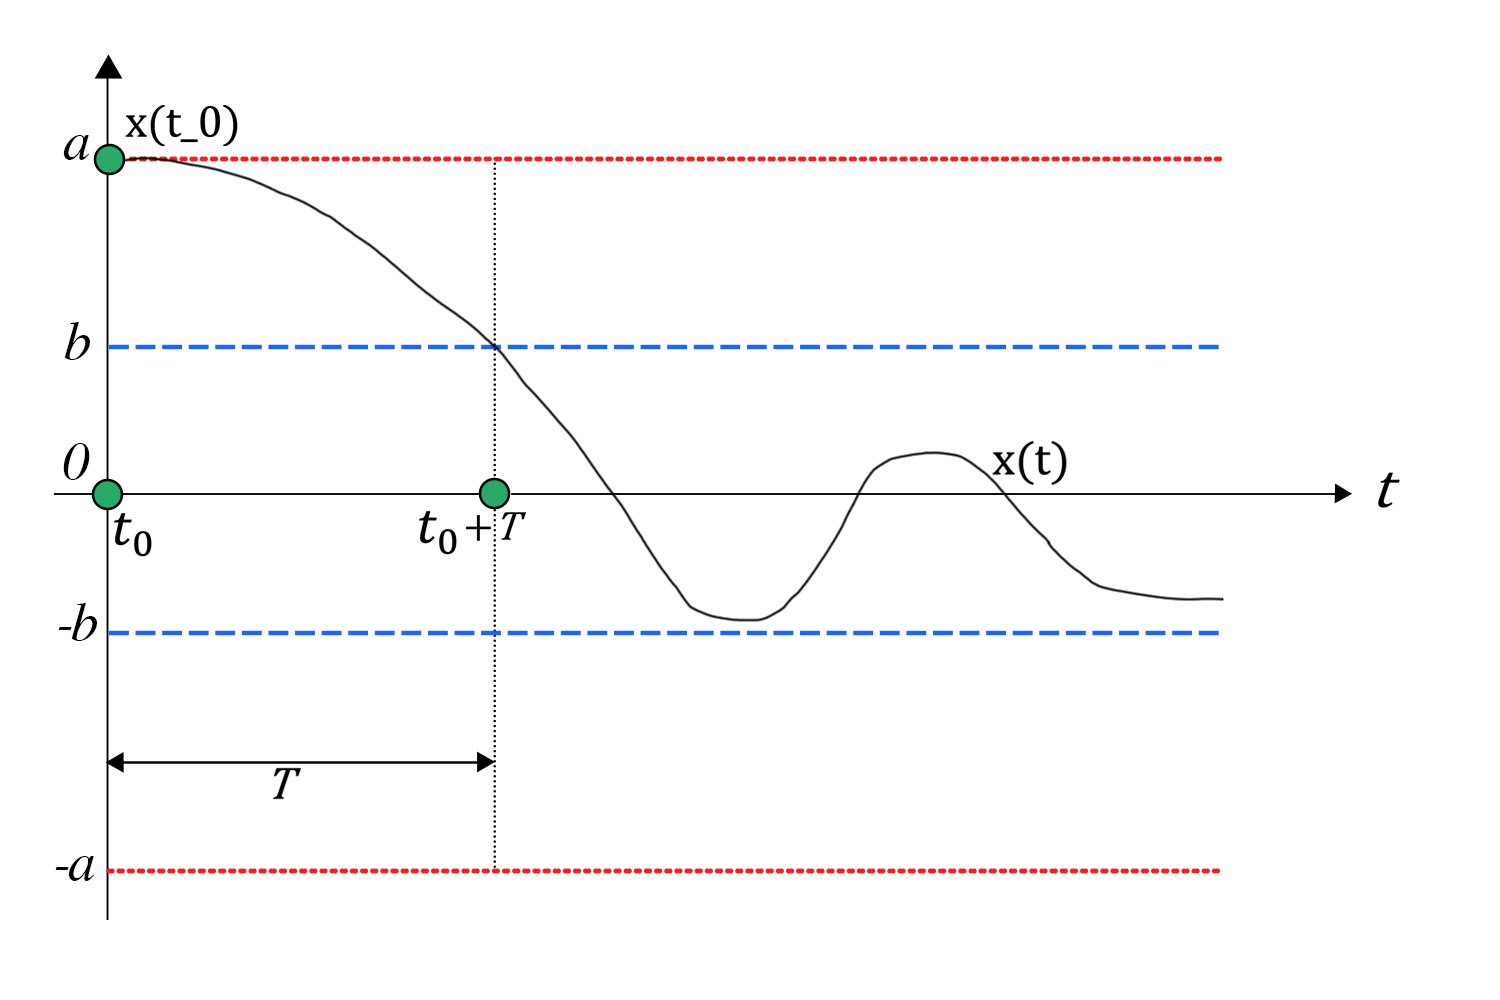
\includegraphics[width=\linewidth]{figures/figure-bounce.jpg}
    \caption{} \label{fig:boundedness_2D}
  \end{subfigure}
  \hspace{4mm}
  \begin{subfigure}[c]{0.31\textwidth}
    \centering
    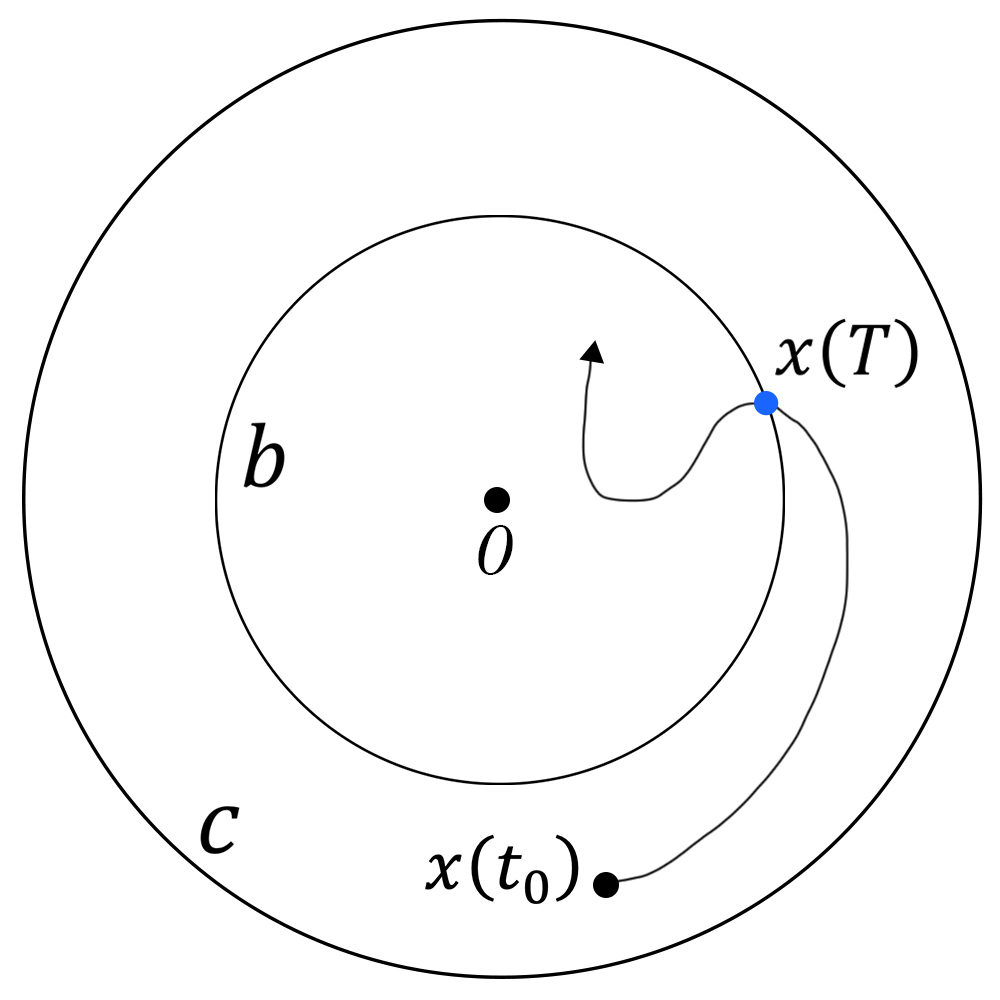
\includegraphics[width=\linewidth]{figures/figure-uub.jpg}
    \caption{} \label{fig:boundedness_3D}
  \end{subfigure}%

  \caption[Visualization of uniform and ultimate boundedness.]{Uniform and ultimate boundedness visualized in 1D (figure \ref{fig:boundedness_2D}) and 2D (figure \ref{fig:boundedness_3D}). In these figures, $t_0$ is the initial time, $T$ the time after the transient period, $x$ the trajectory and $a$ and $b$ are the uniform and ultimate bound, respectively.} \label{fig:boundedness_notions}
\end{figure}

%% Definition - Uniform and ultimate boundedness.
\begin{definition}[list text=Uniform and ultimate boundedness]{Uniform and ultimate boundedness \cite{khalilNonlinearControl2015}}{boundedness}
  The solutions of the \textbf{unforced} (i.e., $u=0$) system \eqref{eq:unforced_nonlinear_system} are
  \begin{itemize}
    \item \textbf{UB} if there	exists $c > 0$, independent of $t_0$, and for every $a \in\left( 0, c \right)$, there is $\beta > 0$, dependent on $a$ but independent of $t_0$, such that
          \begin{equation} \label{eq:uniform_boundedness}
            \left\|x\left(t_0\right)\right\| \le a \Rightarrow \left\|x\left(t \right)\right\| \le \beta, \quad \forall \; t \ge t_0.
          \end{equation}
    \item \textbf{Globally UB} if \eqref{eq:uniform_boundedness} holds for arbitrarily large $a$.
    \item	\textbf{UUB} with ultimate bound $b$ if there exists a positive constant $c$, independent of $t_0$, and for every $a \in\left( 0, c \right)$, there is a $T \geq 0$, dependent on $a$ and $b$ but independent of $t_0$, such that
          \begin{equation} \label{eq:uniform_ultimately_boundedness}
            \left\|x\left(t_0\right)\right\| \le a \Rightarrow \left\|x\left(t \right)\right\| \le b, \quad \forall \; t \ge t_0 + T.
          \end{equation}
    \item \textbf{Globally UUB} if \eqref{eq:uniform_ultimately_boundedness} holds for arbitrarily large $a$.
  \end{itemize}
\end{definition}

It is important to note that in contrast to $\epsilon$ in SISL, here, the (ultimate) bound $b$ can not be made arbitrarily small by starting closer to the equilibrium point of origin. This bound instead depends on the system dynamics, uncertainties and disturbances. As a result, these stability notions can be seen as "milder" forms of SISL. As they are not defined around specific equilibrium points, they only require that trajectories converge to a given bound in finite time and stay therein for all future times (see figure \ref{fig:boundedness_3D}). Therefore, they are easier to achieve in practical dynamical systems subject to uncertainties and disturbances.

Like the other stability notions, a Lyapunov analysis can be used to investigate the UB and UUB of nonlinear systems. Since the Lyapunov conditions used in this analysis are very similar to those in theorem \ref{th:unforced_auto_lyapunov_conditions}, they will not be displayed here. Instead, they can be found in \cite{khalilNonlinearControl2015} with their proof and several examples.

\subsubsection{Stability of perturbed systems}
% NOTE: Theory for this section can be found in \cite{khalilNonlinearSystems2002} section 9.1.

Besides being time-dependent and possibly lacking distinct equilibrium points, real systems can also be subject to perturbations caused by modelling errors, ageing, uncertainties, and disturbances. It turns out that for stable unperturbed systems, Lyapunov's stability theory can be extended to include perturbations when information about these perturbations, like an upper bound, is available. To demonstrate this, let us extend the system of \eqref{eq:unforced_nonlinear_system} with a perturbation $g\left(t, x\right)$:
\begin{equation} \label{eq:perturbed_nonlinear_system}
  \dot{ x }= f \left(x, t, u\right)+ g \left(t, x\right), \quad u = 0.
\end{equation}
Like $f$, $g :\left[0, \infty\right)\times D \rightarrow\mathbb{R}^n$ is also piecewise continuous in $t$ and locally Lipschitz in $x$ and $u$. Further $g$ can be a vanishing (i.e., $g \left( t, 0 \right)= 0$) or non-vanishing (i.e., $g \left(t, 0 \right)\neq 0$). Now suppose that the nominal system \eqref{eq:unforced_nonlinear_system} has an ES equilibrium point $x = 0$, and $V\left(t, x \right)$ is a Lyapunov function that satisfies
\begin{equation}
  c_1 \left\|x\right\|^2 \le V\left(t, x \right) \le c_2 \left\|x \right\|^2,
\end{equation}
\begin{equation} \label{eq:perturbed_lyapunov_condition2}
  \frac{\partial V}{\partial t} + \frac{\partial V}{\partial x}{f \left( t, x \right)} \le - k_3 \left\|x\right\|^2,
\end{equation}
\begin{equation} \label{eq:perturbed_lyapunov_condition3}
  \left\|\frac{\partial V}{\partial x}\right\| \le c_4 \left\|x\right\|,
\end{equation}
for all $\left( t, x \right) \in \left[0, \infty\right) \times D$ for some positive constants $c_1$, $c_2$, $c_3$ and $c_4$. These conditions, which can be seen as the inverse or converse\footnote{More information on the inverse Lyapunov theorems can be found in section 4.7 of \cite{khalilNonlinearSystems2002}.} of the Lyapunov conditions in theorem \ref{th:unforced_auto_lyapunov_conditions}, prove that some $V\left(t, x\right)$ exists, given an ES equilibrium exists.

Now let us assume that we know $g$ is a vanishing perturbation (i.e., $g \left( t, 0 \right)= 0$) which is linearly bounded by
\begin{equation} \label{eq:perturbation}
  \left\|g\left( t, 0 \right)\right\| \le \gamma \left\|x\right\|, \quad \forall \; t \ge 0, \quad \forall \; x \in D,
\end{equation}
in which $\gamma$ is a nonnegative constant. Given this information and the fact that the nominal system has an ES equilibrium point, a natural approach would be to use the Lyapunov function of the nominal system as a candidate for investigating the stability of the perturbed system. Doing this results in the following derivative of $V$ along the trajectories of \eqref{eq:perturbed_nonlinear_system}:
\begin{equation} \label{eq:perturbed_auto_lyap_derivative}
  \dot{ V }\left( t, x \right)=\frac{\partial V}{\partial t} + \frac{\partial V}{\partial x} f \left( t, x \right) + \frac{\partial V}{\partial x} g \left(t, x \right).
\end{equation}
The first two terms on the right-hand side of \eqref{eq:perturbed_auto_lyap_derivative} represent the contribution of the nominal system. Because these terms are always negative definite, the resulting $\dot{V}\left( t, x\right)$ is also negative definite, and condition \eqref{eq:perturbed_lyapunov_condition2} is satisfied. The third term, $\left[\frac{\partial V}{\partial x}\right] g \left(t, x \right)$, represents the effect of the perturbation. Since no exact knowledge is available about $g$ the effect of this term on the definiteness of $\dot{ V }\left( t, x \right)$ is unknown. Therefore, we can at best use the linear bound on $g$, which was given in \eqref{eq:perturbation}, to investigate the worst-case scenario. Using this information with \eqref{eq:perturbed_lyapunov_condition2} and \eqref{eq:perturbed_lyapunov_condition3} results in the following inequality:
\begin{equation}
  \dot{ V }\left( t, x \right) \le - c_3\left\|x\right\|^2 + \left\|\frac{\partial V}{\partial x}\right\|\left\|g\left(t, x\right)\right\| \le -c_3\left\|x\right\|^2+c_4\left\|x\right\|^2.
\end{equation}
From this, we can determine that if $\gamma$ is small enough to satisfy the bound
\begin{equation}
  \gamma<\frac{c_3}{c_4},
\end{equation}
then
\begin{equation}
  \dot{ V }\left( t, x \right) \le - \left( c_3 - \gamma c_4 \right) \|x\|^2, \quad \left(c_3 - \gamma c_4\right) > 0.
\end{equation}
Using Theorem~\ref{th:unforced_auto_lyapunov_conditions} it can therefore be concluded that the origin of the nominal system is also a (globally) ES equilibrium point of the perturbed system. As a result, although the perturbation can disturb the system trajectories away from the equilibrium point, the system will return to this equilibrium point when it is gone. A similar relationship can be derived when the nominal system has an AS equilibrium point \cite{khalilNonlinearControl2015}.

In the case that $g$ is a non-vanishing perturbation, the equilibrium point $x = 0$ of the nominal system \eqref{eq:unforced_nonlinear_system} may no longer be the equilibrium point of the perturbed system \eqref{eq:perturbed_nonlinear_system}. As a result, the reasoning above is no longer valid. For these systems, we can, at best, prove that $x\left(t\right)$ is bounded by a small bound (i.e., UUB) if the perturbation is relatively small. More information about this extension of UB and UUB to non-vanishing perturbed systems can be found in Chapter 9 of \cite{khalilNonlinearSystems2002}.

\subsection{Stability of forced non-autonomous systems}

The previous chapter extended Lyapunov's stability theory to work for unforced, non-autonomous and perturbed systems. In most cases, however, we are not interested in the stability of free or perturbed systems but that of the system when it is being controlled (i.e., $u \neq 0$). Two distinct approaches can be taken for investigating the stability of controlled systems: the state-space approach and the input-output approach. In the state-space approach, a detailed model of the inner structure of the system is used to investigate the behaviour of the state variables. On the other hand, the input-output approach treats the system as a black box and relates the system's output directly to the input. These two approaches seed two distinct stability notions: \textbf{input-to-state stability (ISS)} and \textbf{input-output stability (IOS)}. IOS is used for systems with no exact state model, for example, systems which can only be approximated due to time delays. Since a dynamics model is readily available for robot manipulators, the rest of the text will focus on ISS. However, concepts like dissipativity and passivity, explained below, can also be applied to IOS. Interested readers can check out \cite{khalilNonlinearControl2015} for more information.

\subsubsection{Input-to-state stability}
% NOTE: Theory for this section can be found in \cite{khalilNonlinearControl2015} section 4.4.

Roughly speaking, a system is said to be ISS if it is GAS or GES in the absence of external inputs and the trajectories $x \left( t \right)$ stay bounded for any bounded input $u \left( t \right)$. The mathematical definition naturally follows the previous sections on UB and perturbed systems if we consider the new input u as a bounded disturbance to the unforced system $\dot{ x }= f \left( x, t, 0 \right)$. For this perturbed system, since $u$ is bounded, it might be possible to show that $\dot{ V }$ is negative (semi-)definite outside a ball of radius $\mu$, where $\mu$ depends on the upper bound of $u$ (i.e., $\sup{\left\|u\right\|}$). As a result, we can use the concept of UB to arrive at the formal definition of ISS shown in definition \ref{def:input_to_state_stability}.

%% Definition - Input-state stability
\begin{definition}[list text=Input-to-state stability,after pre=\footnotetext{Definition 4.4 of \cite{khalilNonlinearControl2015} was slightly changed for consistency with the rest of the text.}]{Input-to-state stability \cite{khalilNonlinearControl2015}\footnotemark}{input_to_state_stability}
  The \textbf{forced} (i.e., $u \ge 0$) system \eqref{eq:unforced_nonlinear_system} is \textbf{input-to-state stable} if there exists a class $\mathcal{KL}$ function $\beta$ and a class $\mathcal{K}$ function $\gamma$ such that for any $t_0 \geq 0$, any initial state $x \left( t_0 \right)$, and any bounded input $u\left( t \right)$, the solution $x \left( t \right)$ exists for all $t \geq t_0$ and satisfies
  \begin{equation}
    \left\|x\left(t\right)\right\| \le \max \left\{ \beta\left(\left\|x\left(t_0 \right)\right\|, t-t_0\right), \ \gamma \left(\sup_{t_0 \leq \tau \leq t}{\left\|u\left(\tau \right)\right\|} \right)\right\}, \quad \forall \; t \geq t_0.
  \end{equation}
\end{definition}

Several Lyapunov-based approaches exist in the literature to prove the ISS of systems: dissipativity, robustness margins and classical Lyapunov-like conditions \cite{khalilNonlinearSystems2002,sontagInputtoStateStabilityProperty1995}. Of these approaches, the notion of dissipativity and its special case passivity is especially convenient when working with the interconnected systems often encountered in control.

\subsubsection{Passivity}
% NOTE: Theory for this section can be found in chapter 2 of \cite{baoProcessControlPassive2007} and chapter 3 of \cite{ebenbauerDissipationInequalitiesSystems2009}.

%% Figure - RLC circuit.
\begin{figure}
  \centering
  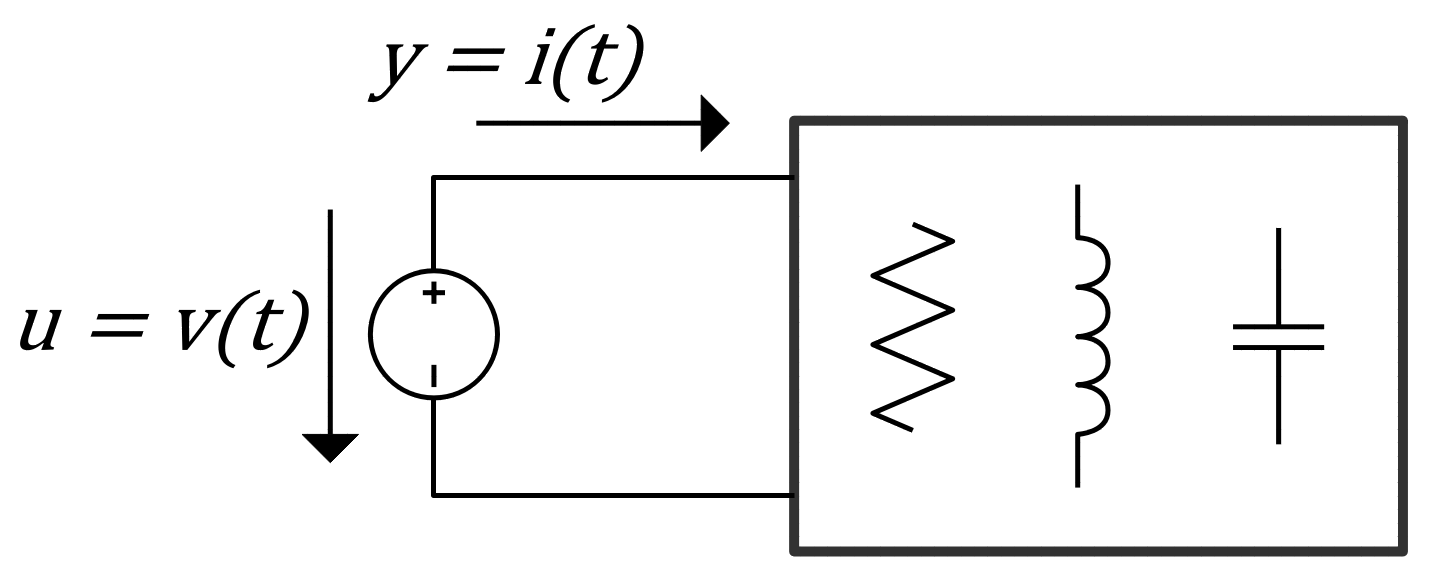
\includegraphics[width=0.55\linewidth]{figures/RLC_circuit.png}
  \caption[Schematic diagram of a general RLC circuit.]{Schematic diagram of a general RLC circuit containing a combination of (passive) resistances, inductors and capacitors. In this, $y$ and $x$ represent the input and output while $v$ and $i$ represent the voltage and current, respectively.} \label{fig:rlc_circuit}
\end{figure}

The concept of a passive system first emerged in the circuit theory field from the energy dissipation in passive component \cite{popovHyperstabilityControlSystems1973}. In electrical networks, an electronic component is called passive if it does not require electrical energy to operate. It can only receive energy from other components and either dissipate, absorb, or store it in an electric or magnetic field. Because of this, networks that only contain passive elements will not generate energy and are, therefore, stable \cite{andersonNetworkAnalysisSynthesis2013}. An example of such a passive network is the general RLC circuit depicted in figure \ref{fig:rlc_circuit}. Since it consists of only passive elements (e.g., inductors, resistors and capacitors), it cannot supply more energy to its environment than it receives. As the power supplied to this network equals the product of voltage and current (i.e., $p \left( t \right)= v \left( t \right) i \left( t \right)$) this results in the following inequality:
\begin{equation}
  E \left( t_1 \right)- E \left( t_0 \right)\le\int_{ t_0 }^{ t_1 } v \left( t \right) i \left( t \right)dt, \quad t_0 \le t_1.
\end{equation}
This inequality which relates the total energy stored in the network $E\left(t\right)$ to the energy supplied to the network, holds for all passive electrical systems.

This notion of passivity was later generalized to other dissipative systems through the introduction of a \textbf{storage function} (energy stored in the system) and a \textbf{supply rate} (externally supplied energy) \cite{willemsDissipativeDynamicalSystems1972a,willemsDissipativeDynamicalSystems1972}. A system is said to be dissipative if its energy (storage function) increases no more than the energy provided (via the supply rate) during a given time interval. This relationship is mathematically expressed in definition \ref{def:dissipativity} below.

%% Definition - Dissipativity.
\begin{definition}[list text=Dissipative system]{Dissipative system \cite{baoProcessControlPassive2007}}{dissipativity}
  System $H$ with \textbf{supply rate} $w \left( t \right)$ is said to be \textbf{dissipative} if there exists a nonnegative real function $S \left( x \right): X \rightarrow\mathbb{R}^+$ called the \textbf{storage function}, such that, for all $t_1 \geq t_0 \geq 0$, $x\left(t_0\right) \in X$ and $u \in U$,
  \begin{equation}
    S \left( x_1 \right)- S \left( x\left(t_0\right) \right) \le \int_{ t_0 }^{ t_1 } w \left( t \right) dt
  \end{equation}
  where $x_1 = \phi \left(t_1, t_0, x\left(t_0\right), u \right)$ and $\mathbb{R}^+$ is a set of nonnegative real numbers.
\end{definition}

In this definition, $H$ can be any general (non-)linear system, while the supply rate $w \left( t \right)$, which determines the type of dissipativity, can be any bounded function defined on the input and output space (i.e., $\int_{ t_0 }^{ t_1 } w \left( t \right)dt<\infty$). If the storage function S is continuously differentiable, this relationship simplifies to
\begin{equation}
  \frac{ dS \left( x \left( t \right)\right)}{ dt }\le w \left( t \right),
\end{equation}
which emphasizes the storage function's positive semi-definiteness. When a bilinear supply rate is used, we receive the general definition of a passive system given in definition \ref{def:passivity}. This definition spans a broad spectrum of passive systems, with \textbf{lossless} and \textbf{state strictly passive} systems being the most extreme cases. Where lossless systems store all energy supplied to them, strictly passive systems lose additional energy due to, for example, heat or friction.

%% Definition - Passivity.
\begin{definition}[list text=Passive system,after pre=\footnotetext{Definition 2.7 of \cite{baoProcessControlPassive2007} was combined with a slightly modified version of definition 5.3 of \cite{khalilNonlinearControl2015}.}]{Passive system \cite{khalilNonlinearControl2015, baoProcessControlPassive2007}\footnotemark}{passivity}
  A system is said to be \textbf{passive} if it is dissipative with respect to the following supply rate:
  \begin{equation}
    w \left(u \left(t\right), y \left( t \right)\right)={ u \left( t \right)}^T y \left( t \right)
  \end{equation}
  and the storage function $S \left( x \right)$ satisfies $S \left( 0 \right)= 0$. Moreover, it is
  \begin{enumerate}
    \item \textbf{Lossless} if $\dot{ S }={ u \left( t \right)}^T y \left( t \right)$.
    \item \textbf{Input strictly passive} if $\dot{S} + {u \left(t \right)}^T \varphi \left(u \left(t \right)\right) \le {u \left(t \right)}^T y \left(t \right) \ and \ {u \left( t \right)}^T \varphi \left(u \left( t \right)\right) > 0, \quad \forall \; u \neq 0$.
    \item \textbf{Output strictly passive} if $\dot{S} + {y \left(t \right)}^T \rho \left(y \left(t \right)\right) \le {u \left(t \right)}^T y \left(t \right) \ and \ {y \left( t \right)}^T \varphi \left(y \left(t \right)\right) > 0, \quad \forall \; u \neq 0$.
    \item \textbf{Strictly passive} if $\dot{S} + \psi \left(x \right) \le {u \left(t \right)}^T y \left(t \right)$ for some positive definite function $\psi$.
  \end{enumerate}
  In all cases, the inequality should hold for all $\left(x, u\right)$. A system that does not adhere to these conditions is said to be \textbf{active}.
\end{definition}

From the definitions above, it is easy to see that the inequality reduces to the aforementioned Lyapunov inequality $\dot{ V }\left( x \left( t \right)\right)\le 0$ when $u = 0$. Because of this, Lyapunov functions, called \textbf{Control Lyapunov functions} for controlled systems, can be used as candidate energy functions in dissipative and passive systems. To better understand the relationship between passivity and stability, let us apply the concept of passivity to the earlier used simple damped pendulum (see example \ref{ex:passivity}).

%% EXAMPLE - Passivity.
% NOTE: Example was based on example 5.5 of \cite{khalilNonlinearControl2015}.
\begin{example}{Passivity analysis of simple damped pendulum}{passivity}
  Consider the simple damped pendulum of example \ref{ex:pendulum}. Let us add an input torque $u$ and rewrite the equations of motion in \eqref{eq:pendulum} as two coupled first-order differential equations:
  \begin{equation} \label{eq:pendulum_state_form}
    \dot{x}_1 = \dot{x}_2, \quad \dot{x}_2 = -\frac{g}{l} \sin(x_1) - \frac{b}{ml^2}x_2 + \frac{1}{ml^2}u,
  \end{equation}
  where $x_1$ is the pendulum angle $\theta$. Now let us take $y = x_2$ as the output and use the expression for the total energy we found in example \ref{ex:pendulum} as a candidate energy function $S$:
  \begin{equation}
    S \left(x_1, x_2 \right) = \frac{1}{2} m l^2 x_2^2 + mgl(1 - \cos{x_1}).
  \end{equation}
  Note that this function is positive semi-definite but not positive definite since it is zero at points other than the origin. Evaluating the time derivative of this energy function gives us
  \begin{equation}
    \dot{S}\left(x_1, x_2\right) = ml x_2 \left( l \dot{x}_2 + g \sin{x_1}\right),
  \end{equation}
  and substituting in the system dynamics from equation \eqref{eq:pendulum_state_form} reveals
  \begin{equation}
    \dot{S}\left(x_1, x_2 \right) = -b x_2 + x_2 u.
  \end{equation}
  Using the passivity relationship in definition \ref{def:passivity} and definition \ref{def:dissipativity} results in the following inequality:
  \begin{equation}
    \dot{S} - u^T y = -b x_2 + x_2 u - u x_2 = -b x_ 2^2 \le x_2 u - u x_2 \le 0.
  \end{equation}
  Hence, the pendulum is \textbf{passive} (i.e lossless) when $b = 0$ and is \textbf{strictly (output) passive} when $b > 0$.
\end{example}

The pendulum example above suggests that passivity implies stability if a positive definite storage function is used. However, passivity does not guarantee stability because the storage function in definition \ref{def:dissipativity} is only required to be positive semi-definite (i.e., nonnegative). This is because the presence of an unobservable unstable part of the system can still destabilise the equilibrium \cite{baoProcessControlPassive2007}. Additional conditions like zero-state detectability and observability, which can be seen as extensions of the invariance principles described above, are required to prove stability through passivity to exclude these situations:

%% Definition - Zero-state detectability and observability.
\begin{definition}[list text=Zero-state detectability and observability]{Zero-state detectability and observability \cite{baoProcessControlPassive2007}}{zero_state}
  A system H is \textbf{zero-state observable (ZSO)} if for any $x \in X$,
  \begin{equation} \label{eq:zero_state_observable}
    y\left(t\right) = h\left(\phi\left(t, t_0, x, u \right)\right) = 0, \quad u = 0, \quad \forall \; t \geq t_0 \geq 0 \quad implies \ x = 0,
  \end{equation}
  and the system is \textbf{locally ZSO} if there exists a neighbourhood $X_n$ of $0$, such that for all $x \in X_n$, \eqref{eq:zero_state_observable} holds. The system is \textbf{zero-state detectable (ZSD)} if for any $x \in X$,
  \begin{equation} \label{eq:zero_state_detectable}
    y\left(t\right) = h\left(\phi\left(t, t_0, x, u\right)\right) = 0, \quad u = 0, \quad \forall \; t \geq t_0 \geq 0 \; implies \lim_{t \rightarrow\infty}{\phi \left(t, t_0, x, 0\right) = 0},
  \end{equation}
  and the system is \textbf{locally ZSD} if there exists a neighbourhood $X_n$ of $0$, such that for all $x \in X_n$, \eqref{eq:zero_state_detectable} holds.
\end{definition}

With these conditions, several relationships between passivity and stability can be derived. The relationships between passivity, SISL and AS are shown in theorem \ref{th:passivity_based_stability}. However, relationships for the other stability notions can also be obtained by modifying the storage function \cite{haddadNonlinearDynamicalSystems2011}. It is important to note that passivity, like Lyapunov stability, is only a sufficient condition for stability, as examples of non-passive systems exist that are stable \cite{ngwompoPassivityAnalysisLinear2017}.
%% Theorem - Passivity based stability conditions.
\begin{theorem}[list text=Passivity based stability,after pre=\footnotetext{Lemma 5.5-5.6 of \cite{khalilNonlinearControl2015} were combined and slightly adjusted for clarity.}]{Passivity based stability \cite{khalilNonlinearSystems2002}\footnotemark}{passivity_based_stability}
  If the \textbf{forced} (i.e., $u \ge 0$) system \eqref{eq:unforced_nonlinear_system} is \textbf{passive} or \textbf{input-strictly passive} with a \textbf{positive definite} storage function $S\left(x\right)$, then the origin of the undisturbed system $x=f\left(t, x, 0\right)$ is \textbf{SISL}. Moreover, it is \textbf{AS} if the system
  \begin{itemize}
    \item \textbf{Strictly passive} or
    \item \textbf{Output strictly passive and ZSO or ZSD}.
          Furthermore, if the storage function is \textbf{radially unbounded}, the origin will be \textbf{GAS}.
  \end{itemize}
\end{theorem}
% QUESTION: The example text can go away.
The discussion above showed that dissipativity and its subclass passivity could be seen as an extension of Lyapunov's stability theory. Where Lyapunov's direct method allows for reasoning about the stability of (unforced) systems, dissipativity also gives information about the input-output relation. In addition, a handy property of passive systems is that passivity is preserved when two passive systems are interconnected in parallel or feedback \cite{haddadNonlinearDynamicalSystems2011}. This makes passivity especially well-suited when working with compositional control designs like controlled robot manipulators. For example, if a passive controller controls a passive manipulator, the resulting combined system is also passive, and the controlled system is guaranteed to never becomes unstable. As a result, Lyapunov's stability theory and the concept of passivity are valuable tools for designing stable controllers for these systems.

\section{Manipulator kinematics/dynamics}

Several formulations are found in the impedance literature describing the dynamics of an $n$-degree of freedom (DOF) manipulator: the Newton-Euler, Euler-Lagrange, and Hamiltonian formulations. The Euler-Lagrange and Hamiltonian formulations are often used in stability research because of their close relationship to the system energy \cite{haddadNonlinearDynamicalSystems2011}, while the Newton-Euler formulation is often used in simulations \cite{sicilianoRoboticsModellingPlanning2010}. In this section, the Euler-Lagrange formulation will be depicted to aid the understanding of the control methods in the next section. More information about the Newton-Euler and Hamiltonian formulations can be found in \cite{sicilianoRoboticsModellingPlanning2010} and \cite{baoProcessControlPassive2007}, respectively. By using this formulation, the joint-space dynamics of a general $n$-DOF robot manipulator operating in an $m$-dimensional Cartesian space can be formulated as
% NOTE: Dynamic relationships retrieved from \cite{sicilianoRoboticsModellingPlanning2010,songTutorialSurveyComparison2019}.
\begin{equation} \label{eq:euler_lagrange}
  M \left( q \right)\ddot{ q }+ C \left( q ,\dot{ q }\right)\dot{ q }+ f \left(\dot{ q }\right)+ g \left( q \right)= u + J^T \left( q \right) F_e,
\end{equation}
where $q \in J \in\mathbb{R}^n$ are the joint positions, $M \in\mathbb{R}^{n \times n}$ represents the inertia matrix, $C \in\mathbb{R}^{ n \times n }$ gives the contributions due to coriolis and centripetal forces, while $g \in\mathbb{R}^n$ and $f \in\mathbb{R}^n$ are the torques due to gravity and friction forces, respectively. Further, $F_e \in\mathbb{R}^m$ denotes a vector of forces and moments exerted on the end-effector by the environment, $J \in\mathbb{R}^{ m \times n }$ the geometric jacobian\footnote{The geometric Jacobian relates the joint velocities $\dot{q}$ to the end-effector linear $\dot{x}_e$ and angular $\omega_e$ velocities using the geometry of the manipulator. More information can be found in section 3.1 of \cite{sicilianoRoboticsModellingPlanning2010}.} and $u \in\mathbb{R}^n$ the joint actuation (i.e., control) torques. Although equation \eqref{eq:euler_lagrange} is expressed in the joint space $\mathcal{J}$, it can also be converted to the task space $\mathcal{C}$ using the following kinematic relationships:
% NOTE: Kinematic relationships retrieved from \cite{al-shukaActiveImpedanceControl2018}.
\begin{equation}
  \dot{ x }_e = J_A \left(q\right)\dot{q},
\end{equation}
\begin{equation}
  J_A \left( q \right)=\frac{\partial k\left( q \right)}{\partial q},
\end{equation}
\begin{equation}
  \ddot{ x }_e = J_A \left( q \right)\ddot{ q } + \dot{ J }_A \left( q ,\dot{ q }\right)\dot{ q },
\end{equation}
in which $x_e \in C \in\mathbb{R}^m$ are the Cartesian positions of the end effector, $k : \mathbb{R}^n \rightarrow\mathbb{R}^m$ the forward kinematics and $J_A \in\mathbb{R}^{ m \times n }$ the analytical Jacobian\footnote{The analytical Jacobian relates the joint velocities $\dot{q}$ to the translational $\dot{x}_e$ and rotational $\phi_e$ velocities of the end-effector frame through direct differentiation of the manipulator kinematics. More information can be found in 3.6 of \cite{sicilianoRoboticsModellingPlanning2010}.}. If we assume $n = m$ and we neglect the joint friction torques, the cartesian space dynamic model becomes\footnote{The full derivation can be found in section 7.8 of \cite{sicilianoRoboticsModellingPlanning2010}.}
% NOTE: Cartesian dynamical model was retrieved from \cite{sicilianoRoboticsModellingPlanning2010} and and the lecture notes of Robotics 2 (see http://www.diag.uniroma1.it/deluca/rob2_en.php).
\begin{equation} \label{eq:euler_lagrange_cartesian}
  M_x \left( q \right)\ddot{ x }_e + C_x \left( q ,\dot{ q }\right)\dot{ x }_e + g_x \left( q \right)= J_ A^{- T }\left( q \right) u + F_a ,\
\end{equation}
where
\begin{equation}
  M_x \left( q \right)= J_ A^{- T }\left( q \right) M \left( q \right) J_ A^{- 1 }\left( q \right),
\end{equation}
\begin{equation}
  C_x \left( q ,\dot{ q }\right)= J_ A^{- T }\left( q \right) C \left( q ,\dot{ q }\right) J_ A^{- 1 }\left( q \right)- M_x \left( q \right)\dot{ J }_A \left( q \right) J_ A^{- 1 }\left( q \right),
\end{equation}
\begin{equation}
  g_x \left( q \right)= J_ A^{- T }\left( q \right) g \left( q \right),
\end{equation}
\begin{equation}
  F_A = T_A^{-T}\left( x_e \right) F_e,
\end{equation}
and $F_A$ is a vector of equivalent forces and moments in the frame of the analytic Jacobian, while $T_A$ is the transformation matrix between the geometric and analytic Jacobian.

\section{Indirect force control}
% NOTE: Literature for this section is found in \cite{sicilianoRoboticsModellingPlanning2010,al-shukaActiveImpedanceControl2018} and the lecture notes of Robotics 2 (see http://www.diag.uniroma1.it/deluca/rob2_en.php).

Now that we have a clear picture of stability, passivity, and the manipulator model, we are ready to introduce indirect force control methods like impedance and its reciprocal admittance. As the name implies, indirect force control methods do not directly control desired reaction forces like force control does but instead enforce them indirectly via reference models. These reference models produce a desired dynamic interaction between the manipulator and its (unknown) environment.

\subsection{Impedance control}

% FIGURE - Impedance control.
\begin{figure}
  \centering
  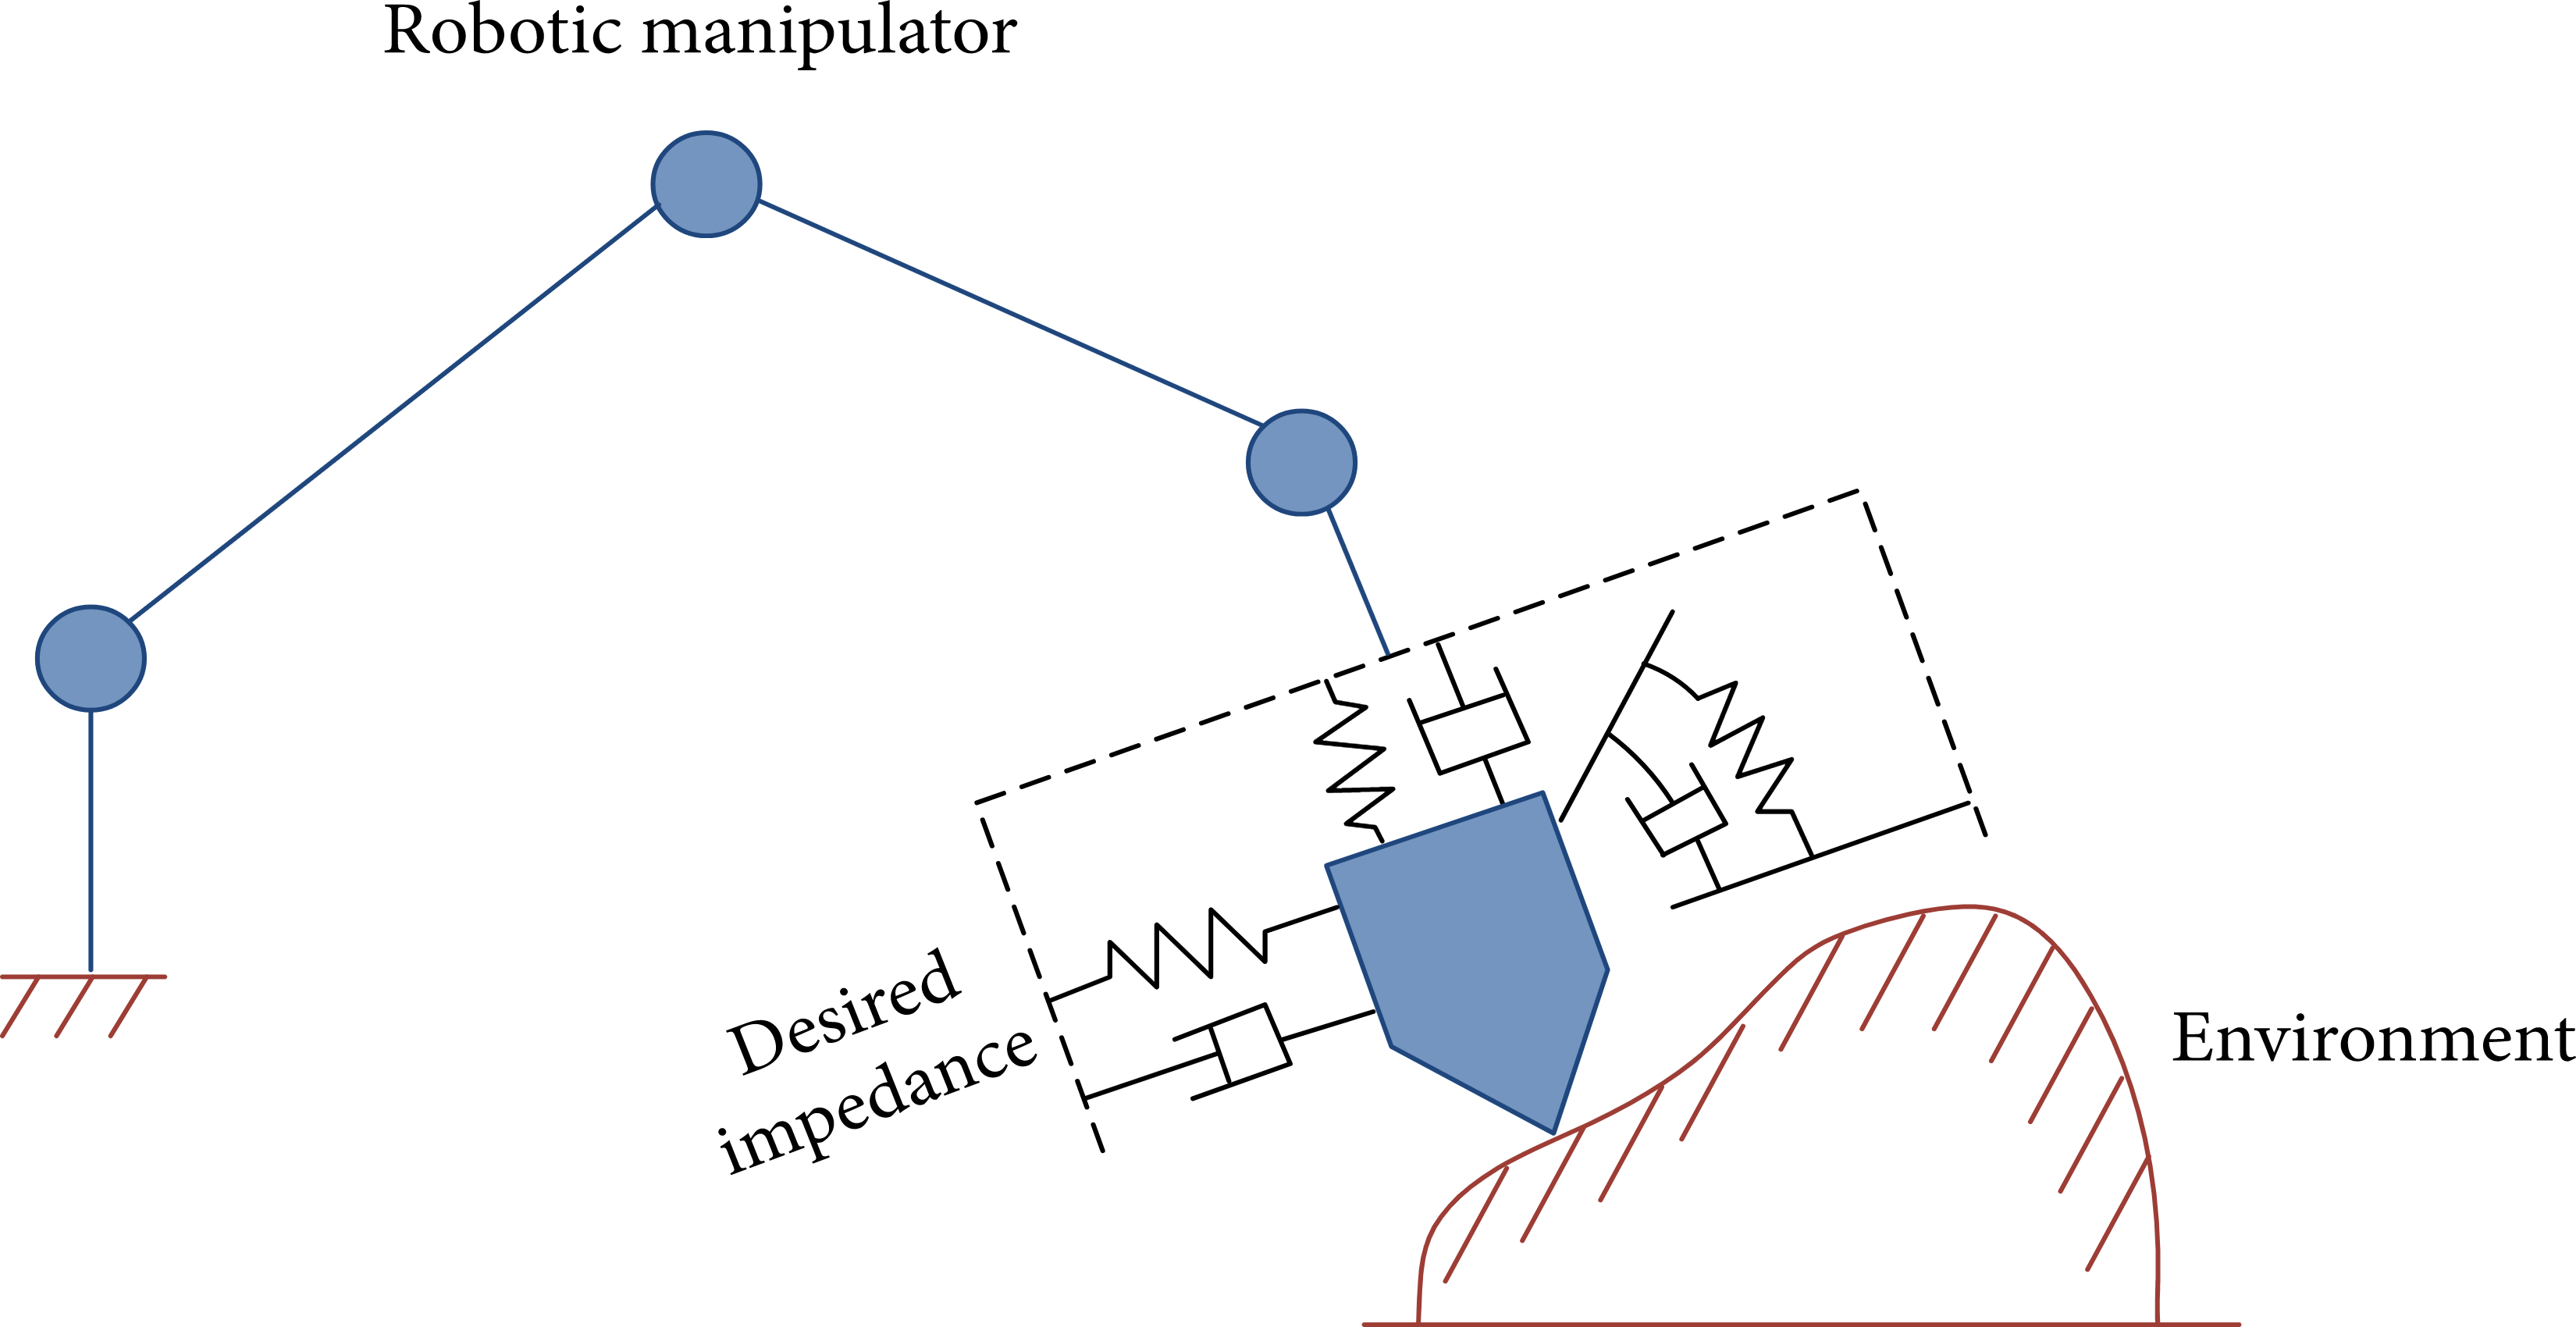
\includegraphics[width=0.5\linewidth]{figures/alshuka_2018.png}

  \caption[Impedance controlled manipulator in contact with the environment.]{Visual representation of impedance control in contact with the external environment \cite{al-shukaActiveImpedanceControl2018}.} \label{fig:impedance_control}
\end{figure}

In impedance control, the desired robot-environment interaction is modelled as a spring-damper system (see figure \ref{fig:impedance_control}) and is generally expressed\footnote{This relationship can also be expressed in the joint space \cite{tsetserukouISoRAHumanoidRobot2009,liImpedanceControlMultipoint2011,liModelfreeImpedanceControl2011,liLearningImpedanceControl2012}. This representation was omitted here since the cartesian version offers more intuition due to its close relationship to the task space.} as
\begin{equation} \label{eq:impedance_relationship}
  M_d \left(\ddot{ x }_e -\ddot{ x }_d \right)+ B_d \left(\dot{x}_e - \dot{x}_d \right)+ K_d \left( x_e - x_d \right) = M_d \ddot{\widetilde{ x }}+ B_d \dot{\widetilde{ x }}+ K_d \widetilde{ x }= F_a,
\end{equation}
in which $x_e$, $\dot{x}_e$, and $\ddot{ x }_e \in\mathbb{R}^n$ are the current position, velocity and acceleration of the manipulator's end effector in the cartesian coordinates, respectively, while the subscript $d$ denotes their desired values. Further, $F_a$ denotes the vector of external forces and torques affecting the system as expressed in the frame of the analytic Jacobian, and $M_d$, $B_{d}$ and $K_d \in\mathbb{R}^{ n \times n }$ are the inertia, damping and stiffness matrices of the desired impedance relationship, respectively, all of which are symmetric and nonnegative definite. This general impedance relationship, called the second-order impedance, can also be simplified to its first or zero-order form by setting the $\ddot{x}_d$ and $\dot{x}_d$ to zero, respectively.

This desired impedance relationship can be enforced on the environment interaction through feedback linearization. Feedback linearization, also called dynamic inversion control, is a control technique that transforms a nonlinear system into a linear system by cancelling out (or compensating) the nonlinear terms. The manipulator model in \eqref{eq:euler_lagrange_cartesian} can be feedback linearized in the cartesian space using the following control law:
\begin{equation} \label{eq:impedance_control_step1}
  u = J_ A^T \left( q \right)\left[ M_x \left( q \right) y + C_x \left( q ,\dot{ q }\right)\dot{ x }_e + g_x \left( q \right)- F_a \right].
\end{equation}
Applying this control law to \eqref{eq:euler_lagrange_cartesian} gives us a linear and decoupled closed-loop system
\begin{equation} \label{eq:impedance_control_step2}
  \ddot{ x }_e = y,
\end{equation}
where $y$ represents a new input vector that directly influences, with a double integrator, the independent cartesian coordinates $x$. This input allows us to enforce any dynamic relationship onto the controlled robot manipulator. By setting $y$ equal to
\begin{equation} \label{eq:impedance_control_step3}
  y = \ddot{ x }_d + M_ d^{- 1 }\left[- B_d \dot{\widetilde{ x }}- K_d \widetilde{ x }+ F_a \right],
\end{equation}
we end up with the impedance model given in \eqref{eq:impedance_relationship}. Combining and simplifying \eqref{eq:impedance_control_step3} and \eqref{eq:impedance_control_step1} gives us the general impedance control law:
\begin{equation}
  \begin{split}
    u = M \left( q \right) J_ A^{- 1 }\left( q \right)\left\{\ddot{ x }_d - \dot{ J }_A \left( q \right)\dot{ q } +  M_ d^{- 1 }\left[- B_d \dot{\widetilde{ x }} - K_d \widetilde{ x }\right]\right\} \\
    +\ C \left( q ,\dot{ q }\right)\dot{ q } + g \left( q \right) + J_ A^T \left( q \right)\left[ M_x \left( q \right) M_ d^{- 1 }- I \right] F_A.
  \end{split}
\end{equation}
This control law, sometimes called \textbf{torque-based impedance control}, produces forces in response to changes in motion and can, therefore, directly be applied to effort-controlled manipulators (see figure \ref{fig:force_based_impedance_control}) or through an optional inner force control loop \cite{al-shukaActiveImpedanceControl2018}. When an accurate model of the robot dynamics (i.e., $M \left( q \right)$, $C \left( q, \dot{ q }\right)$ and $g \left( q \right)$) and a measurement of the external forces and torques $F_a$ are available, it allows precise shaping of the environment interaction using the impedance parameters $M_d$, $B_d$, $K_d$. Of these, $M_d$ influences the control system's response speed, $B_D$ the shape of the transient behaviours and $K_d$ the trade-off between contact forces and free space position accuracy.

% FIGURE - Force-based impedance control schedule.
\begin{figure}
  \centering
  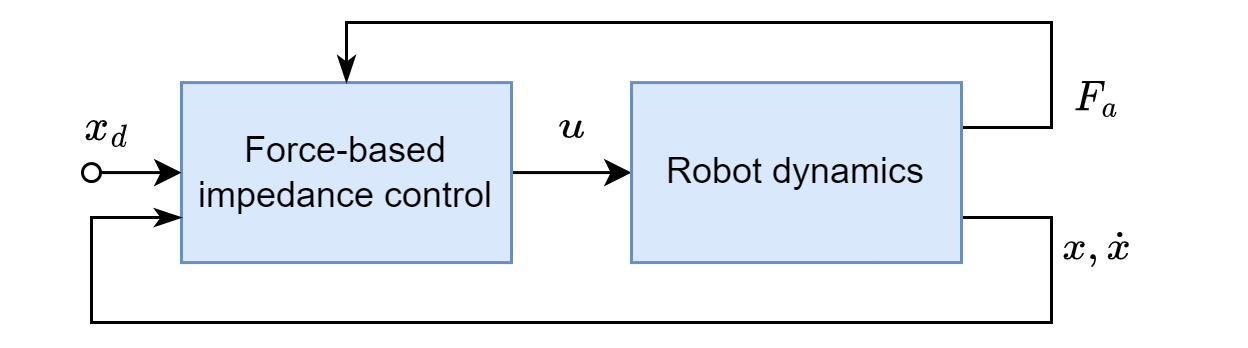
\includegraphics[width=0.65\linewidth]{figures/force_impedance.png}

  \caption[Force-based impedance control diagram.]{Schematic diagram of force-based impedance control. In this figure, $x$ and $\dot{ x }$ are the current position and velocity, respectively, $x_d$ is the desired position, $u$ the control command and $F_a$ the external forces and torques \cite{ottCartesianImpedanceControl2008}.} \label{fig:force_based_impedance_control}
\end{figure}

\subsubsection{Cartesian stiffness control}

The general impedance model above can only be used when a measurement of the external force $F_a$ is available. In some cases like robotic surgery, however, placing a force sensor at the robot end-effector can be difficult \cite{ferragutiTankbasedApproachImpedance2013}. It turns out that impedance control can also be used in these situations if we modify \eqref{eq:impedance_relationship} so that the desired inertia $M_d$ is equal to the actual inertia of the robot $M_x\left( q \right)$:
\begin{equation}
  M_x \left( q \right)\ddot{\widetilde{ x }}+ \left( B_d + C \left( q ,\dot{ q }\right)\right)\dot{\widetilde{ x }}+ K_d \widetilde{ x } = F_a,
\end{equation}
where $C \left( q ,\dot{ q }\right)$ was introduced to preserve the mechanical properties of the configuration-dependent inertia $M_x \left( q \right)$. Applying this new impedance model through feedback linearization results in the following control law:
\begin{equation}
  u = M\left(q \right)J_A^{-1}\left(q\right)\left\{\ddot{x}_d - \dot{J}_A \left(q\right)J_A^{-1}\left(q\right)\dot{x}_d\right\} + C \left(q,\dot{q}\right)J_A^{-1}\left(q\right)\dot{x}_d + g \left( q \right) - J_ A^T \left( q \right)\left[B_d\dot{\widetilde{ x }} + K_d \widetilde{ x }\right].
\end{equation}
This new control law, called \textbf{cartesian stiffness control}, is similar to a pure motion control law but designed to keep limited contact forces at the end-effector level. It no longer has a dependency on the contact forces $F_a$ and can therefore be used without a measurement of this force. However, it has two drawbacks: first, we lose the ability to change the system's behaviour using the desired inertia $M_d$, and second, because of the presence of the extra $C \left( q ,\dot{ q }\right)$, it can only be used at low velocities.

\subsubsection{Admittance control}

% FIGURE - Position-based impedance control schedule.
\begin{figure}
  \centering
  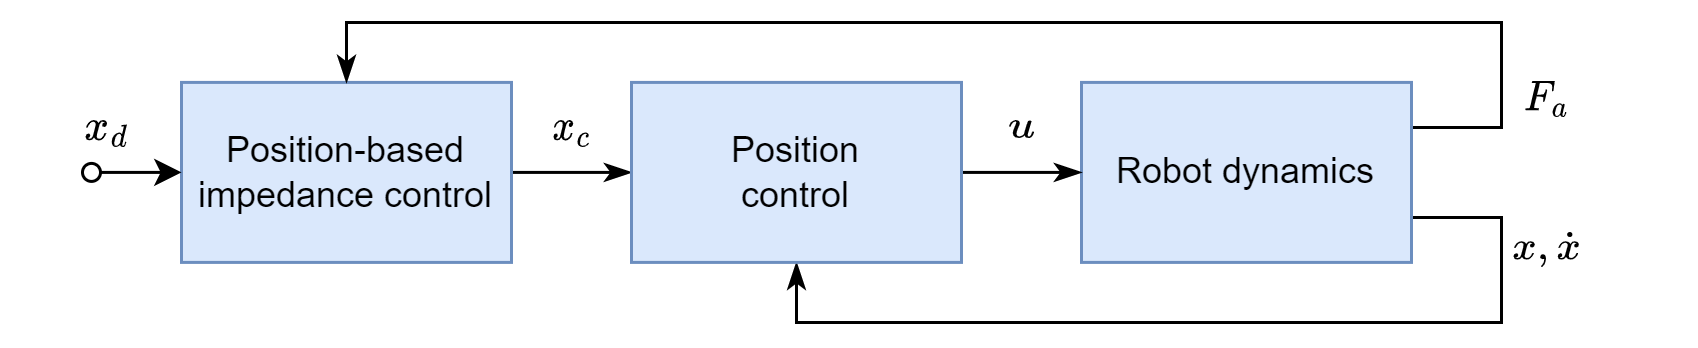
\includegraphics[width=0.9\linewidth]{figures/position_impedance.png}

  \caption[Position-based impedance control diagram.]{Schematic diagram of a position-based impedance controller. In this figure, $x$ and $\dot{ x }$ are the current position and velocity, respectively, $x_d$ is the desired position, $x_c$ the reference position, $u$ the control command and $F_a$ the external forces and torques \cite{ottCartesianImpedanceControl2008}.} \label{fig:position_based_impedance_control}
\end{figure}
As mentioned above, a trade-off exists between contact forces and free space position accuracy in general impedance control. In the absence of interaction (i.e., free motion), impedance control becomes equivalent to inverse dynamics position control, and therefore a high $K_d$ is needed for robustness against disturbances or model uncertainties. This high $K_d$ will, however, lead to undesired high impact forces when in contact. \textbf{Position-based or velocity-based impedance control} provides a solution to this trade-off by splitting the control into two control loops: an inner loop that controls (compliant) position or velocity references and an outer loop that provides these references based on the desired target impedance dynamics (see figure \ref{fig:position_based_impedance_control} for a general description). A simple proportional-integral-derivative (PID) can be used for the inner control loop, while a modified version of the impedance model in \eqref{eq:impedance_relationship} is used for the outer control loop:
\begin{equation}
  M_d \left(\ddot{ x }_c -\ddot{x}_d \right)+ B_d \left(\dot{ x }_c - \dot{ x }_d \right)+ K_d \left( x_c - x_d \right)= F_a,
\end{equation}
where $x_c$, $\dot{ x }_c$, and $\ddot{ x }_c \in\mathbb{R}^n$ now are the reference position, velocity and acceleration, respectively. This type of control, which generates reference motions $x_c$ in response to contact forces $F_a$, is also known as \textbf{admittance control} because of its close resemblance to mechanical admittance. It is often used for interaction tasks dealing with compliant environments or free space, while impedance control is often used for interactions with stiff environments.

\subsubsection{Variable impedance control}
\label{section:variable_impedance_control}

Although the general impedance model in \eqref{eq:impedance_relationship} allows us to design the interaction with the environment precisely, it is still restrictive since this interaction can not be changed during the motion. It is, therefore, only suited for simple tasks where the environment stiffness is constant and can not be used to track desired contact forces. In contrast, humans change their muscle stiffness during motion to attenuate any disturbances or track desired interaction forces \cite{tomoriVariableImpedanceControl2013}. Doing this allows them to perform complex interaction tasks in changing and uncertain environments while precisely controlling the force applied to these environments. The general impedance model in \eqref{eq:impedance_relationship} can be extended to match this human behaviour by allowing the impedance parameters $M_d$, $B_d$ and $K_d$ to vary. This results in the following impedance model:
\begin{equation} \label{eq:variable_impedance}
  M_d\left(t \right)\ddot{\widetilde{ x }} + B_d \left( t \right)\dot{\widetilde{ x }} + K_d \left( t \right)\widetilde{ x }= F_a,
\end{equation}
in which the impedance parameters $M_d \left( t \right), \ B_d \left( t \right)\ and\ K_d \left( t \right)$ are now a function of time. As stated in the introduction, however, this \textbf{variable impedance control (VIC)} model destroys the passivity of the system unless a proper impedance profile is selected. To prove this, let us assume the desired inertia $M_d$ is constant while the desired damping $B_d$ and stiffness $K_d$ are allowed to change with time. Using the following positive definite Lyapunov function:
\begin{equation}
  V \left(\widetilde{ x }, \dot{\widetilde{ x }}\right)=\frac{ 1 }{ 2 }{\dot{\widetilde{ x }}}^T M_d \dot{ x }+\frac{ 1 }{ 2 }{\widetilde{ x }}^T K \left( t \right)\widetilde{ x }
\end{equation}
and taking its derivative while substituting $\ddot{ x }$ from \eqref{eq:variable_impedance} gives
\begin{equation} \label{eq:variable_impedance_derivative}
  \dot{V} = \dot{\widetilde{x}}^T F_a + \left[\frac{1}{2}\widetilde{x}^T \dot{K_d}\left(t \right)\widetilde{ x }-\dot{\widetilde{ x }}^T B_d \left( t \right)\dot{\widetilde{ x }}\right].
\end{equation}
From this derivative, since the sign of the term between the brackets is undefined, it is apparent that the passivity condition of definition \ref{def:passivity} only holds when the stiffness is constant or decreasing $\dot{V} \le \dot{\widetilde{x}} F_a$. As a result, energy might be injected into the system when the stiffness increases, possibly making it unstable. A similar conclusion can be drawn for the case where the inertia is also allowed to vary.

\subsection{Limitations}

While the indirect force control methods above, compared to direct force control methods, are better suited to handle interaction tasks, they also have one major drawback. Due to the use of feedback linearization, an accurate model of the system is required. They are, therefore, not suited in situations where this model is unavailable or significantly impacted by model uncertainties, disturbances or other noises. If so, more advanced indirect control methods like robust or adaptive impedance control can be used \cite{songTutorialSurveyComparison2019,khalilNonlinearControl2015,villaniForceControl2016}.

\section{Further reading}

This chapter is intended to be a quick primer on stability, passivity, and impedance control. Readers can check out \cite{bacciottiStabilityControlLinear2019} for more information on stability criteria and control methods used with linear systems. For nonlinear systems, an excellent introduction to the control of nonlinear systems is given by \cite{khalilNonlinearControl2015}, while \cite{khalilNonlinearSystems2002} serves as a deep dive into all the stability proofs and more advanced methods. Further, \cite{baoProcessControlPassive2007} is an excellent introduction to passivity-based control, while \cite{haddadNonlinearDynamicalSystems2011} covers more advanced concepts. Lastly, readers are referred to \cite{sicilianoRoboticsModellingPlanning2010} for a detailed explanation of impedance control, while recent reviews of impedance research are found in \cite{songTutorialSurveyComparison2019} and \cite{al-shukaActiveImpedanceControl2018}.
